\documentclass{article}
\usepackage{graphicx} % Required for inserting images
\usepackage[dvipsnames]{xcolor}
\usepackage{changepage} % required for adjustwidth
\usepackage{soul} % required for \ul, underline doesn't wrap
\usepackage{color, colortbl}
\usepackage{longtable}
\usepackage{tabu}
\usepackage{tabularray}
\usepackage{siunitx}  % required for \num 
\usepackage{enumitem}% http://ctan.org/pkg/enumitem
\usepackage{fmtcount}
\usepackage{pifont,amssymb} % for the symbols
\usepackage{listings} % parti di codice sql
\usepackage{ulem} % dasuline

\lstset{ % listings config
  % basicstyle=\ttfamily,
  % emphstyle=\textbf
  columns=fullflexible,
  frame=single,
  breaklines=true,
  postbreak=\mbox{\textcolor{red}{$\hookrightarrow$}\space},
}
% \usepackage[shortlabels]{enumitem}
\graphicspath{ {./images/} }
% le prossime 4 righe rendono doc cartella default per input
% \makeatletter
% \providecommand*{\input@path}{}
% \edef\input@path{{./doc/}\input@path}% prepend
% \makeatother

\def\indent1{0.3cm}
\newcommand{\speciale}[1]{\textbf{\textcolor{blue}{\ul{#1}}}}
\newcommand{\specialeb}[1]{\textit{\textcolor{ForestGreen}{\dashuline{#1}}}}


	
\definecolor{Gray}{gray}{0.9}
\definecolor{PaleGreen}{RGB}{152,251,152}
\definecolor{SkyBlue}{RGB}{135,206,235}
\definecolor{PaleTurquoise}{RGB}{179,238,238}
\definecolor{MediumAquamarine}{RGB}{102,205,170}
\definecolor{ColdPurple}{RGB}{171, 160, 217}
\definecolor{LightCoral}{RGB}{240, 128, 128}
\definecolor{CornflowerBlue}{RGB}{100, 149, 237}
\definecolor{PalePink}{RGB}{253, 215, 244}

\newlist{answerlist}{enumerate}{2}
\setlist[answerlist]{label={\alph*.\makebox[0pt][r]{\noexpand\emptysquare\hspace{2em}}},ref=\alph*}

\newcommand{\emptysquare}{$\square$}
\newcommand{\checkedsquare}{\makebox[0pt][l]{\raisebox{1pt}[0pt][0pt]{\large\hspace{1pt}\cmark}}$\square$}
\newcommand{\cmark}{\ding{51}}%
\newcommand{\correctanswer}{{\renewcommand{\emptysquare}{\checkedsquare}\item\leavevmode}}


% https://erd.dbdesigner.net/designer/schema/1721817964-basi-di-dati

%%%%%%%%%%%%%%%%%
% DOC BEGINS HERE
%%%%%%%%%%%%%%%%%

\title{Relazione Basi di Dati}
\author{
  Dobrianskiy, Sergio \\
  \texttt{sergio.dobrianskiy@studio.unibo.it}\\
  \texttt{0001019553}
  \and
  Rigato, Valentina\\
  \texttt{valentina.rigato@studio.unibo.it}\\
  \texttt{0001027266}
}
\date{01 Marzo 2024}

\begin{document} 
\maketitle

\includegraphics[width=0.95\columnwidth]{CesenaCard2.png}
\newpage

\tableofcontents
\clearpage

\section{Introduzione}
L’obiettivo del progetto è di realizzare un servizio web di acquisto e utilizzo di una carta elettronica chiamato CityCard.
CityCard è un sistema che favorisce l’interazione tra turisti e fornitori. Con fornitore si intende chiunque organizzi eventi o fornisca servizi.
I servizi e gli eventi proposti saranno a discrezione dei fornitori, ma potranno spaziare dalla vendita di visite guidate a spettacoli teatrali. 
Servizi ed eventi si distinguono in quanto i primi saranno ad occorrenza singola e avranno un costo mentre gli eventi saranno gratuiti e avranno la possibilità di essere periodici.
Inoltre la CityCard permette fornisce l'accesso gratuito a tutti i mezzi di trasporto pubblico della zona interessata.

Per accedere al sito web i clienti dovranno creare un account fornendo le loro generalità. Una volta registrato l’utente base potrà attivare una CityCard che avrà una validità limitata. 
Ogni CityCard avrà associato un cliente e una carta di credito predefinita con e dovrà venire attivata sottoscrivendo un abbonamento. 
L'abbonamento, oltre a permettere partecipare ad eventi, comprare servizi e l'utilizzo dei trasporti pubblici, fornirà uno sconto sul prezzo dei servizi. 


Si prevede l'esistenza di tre tipi di account: cliente, fornitore, admin.

All’interno del portale web il cliente potrà vedere una lista degli eventi, dei servizi disponibili ed effettuare il check-in sui trasporti pubblici. 
L'utente, inoltre, avrà la possibilità di lasciare una recensione per il servizio acquistati.

I fornitori potranno invece creare enti, associarsi ad uno di essi, rendere disponibili servizi ed eventi, e visualizzare statistiche relative all'ente al quale sono associati.

Gli account degli amministratori potranno visualizzare gli utenti registrati e in caso bannarli, visualizzare gli enti registrati e resettare le loro recensioni, e consultare statistiche relative al servizio.


\section{Analisi dei requisiti}

\subsection{Requisiti in linguaggio naturale}
La seguente descrizione riporta in linguaggio naturale i requisiti per il nostro sistema informativo:

\begin{adjustwidth}{\indent1}{\indent1}
"La software house CityNet© richiede un sistema informativo per la gestione del servizio CityCard che consenta agli utenti di acquistare abbonamenti e accedere a servizi ed eventi forniti da enti affiliati. CityCard può essere emessa sia in formato fisico che virtuale (online) e ha una durata di 5 anni, l'emissione della carta è gratuita e ogni utente ne può avere attiva al massimo una.
L'utilizzo della CityCard necessita la sottoscrizione di un abbonamento a scelta tra tre tipologie, ciascuna con una durata e un prezzo specifici. 
L'abbonamento permette agli utenti di acquistare servizi o prenotare eventi forniti dagli enti partner con uno sconto che varia dalla durata dell'abbonamento.

Il servizio deve essere fornito su un sito al quale l'utente si deve registrare.

Gli utenti si suddividono in tre categorie: cliente, fornitore e admin o amministratore. Una persona può creare più di un account.

Gli enti sono gestiti da utenti di tipo "fornitore", i quali, una volta associati a un ente, hanno la possibilità di creare nuovi servizi o eventi. 

Al primo login gli utenti di tipo "cliente" possono solamente ottenere una CityCard e gestire le carte di credito. Dopo l'attivazione potranno accedere anche alla sezione abbonamenti. Una volta sottoscritto l'abbonamento potranno accedere a tutti i servizi.

I clienti potranno aggiungere più di una carta di credito e renderne una predefinita per i pagamenti.
I clienti possono acquistare i servizi forniti utilizzando la carta di credito predefinita e godendo dello sconto già nominato in precedenza. La CityCard permette anche di partecipare agli eventi gratuiti e di usufruire gratuitamente del trasporto pubblico. 
I clienti, inoltre, avranno la possibilità di lasciare una recensione sui servizi acquistati.

L'utente di tipo "admin" ha la facoltà di bannare gli altri utenti, resettare le recensioni di un ente e visualizzare statistiche globali.

L'utente di tipo "fornitore" deve poter creare enti nuovi, associarsi ad uno di essi, creare servizi ed eventi e visualizzare statistiche dell'ente con il quale è associato.

Tutti gli utenti devono poter aggiornare le informazioni del proprio account.

Gli eventi devono essere singoli o periodici. 

Si deve tenere traccia dei check-in falliti.

Il sistema dovrà essere progettato per garantire una gestione efficace delle diverse funzionalità descritte, assicurando un'esperienza utente intuitiva e fluida per tutte le tipologie di utenti."
\end{adjustwidth}

\subsection{Estrazione dei concetti fondamentali}
\subsubsection{Entità e Attributi}
Lo schema va analizzato per individuarne le parole e le espressioni chiave, con queste verrà realizzato un primo schema riassuntivo che verrà raffinato in seguito. I termini di rilievo appaiono nel testo con un colore diverso:

\begin{adjustwidth}{\indent1}{\indent1}
"La software house CityNet© richiede un sistema informativo per la gestione del servizio \speciale{CityCard} che consenta agli \speciale{utenti} di \specialeb{acquistare} \speciale{abbonamenti} e \specialeb{accedere} a \speciale{servizi} ed \speciale{eventi} forniti da \speciale{enti} affiliati. \speciale{CityCard} può essere \specialeb{emessa} sia in formato fisico che virtuale (online) e ha una durata di 5 anni, l'\specialeb{emissione} della carta è gratuita e ogni \speciale{utente} ne può avere attiva al massimo una.

L'utilizzo della \speciale{CityCard} necessita la \specialeb{sottoscrizione} di un \speciale{abbonamento} a scelta tra tre \speciale{tipologie}, ciascuna con una durata e un prezzo specifici. L'\speciale{abbonamento} permette agli \speciale{utenti} di \specialeb{acquistare} \speciale{servizi} o \specialeb{prenotare} eventi forniti dagli \speciale{enti} partner con uno \speciale{sconto} che varia dalla \speciale{durata} dell'abbonamento.
Il servizio deve essere fornito su un \speciale{sito} al quale l'\speciale{utente} si deve \specialeb{registrare}.

Gli utenti si suddividono in tre categorie: \speciale{cliente}, \speciale{fornitore} e \speciale{admin} o \speciale{amministratore}. Una persona può \specialeb{creare} più di un \speciale{account}.

Gli \speciale{enti} sono gestiti da \speciale{utenti} di tipo "\speciale{fornitore}", i quali, una volta \specialeb{associati} a un \speciale{ente}, hanno la possibilità di \specialeb{creare} nuovi \speciale{servizi} o \speciale{eventi}. 

Al primo \specialeb{login} gli \speciale{utenti} di tipo "\speciale{cliente}" possono solamente \specialeb{ottenere} una \speciale{CityCard} e \specialeb{gestire} le \speciale{carte di credito}. Dopo l'\specialeb{attivazione} potranno accedere anche alla sezione \speciale{abbonamenti}. Una volta \specialeb{sottoscritto} l'\speciale{abbonamento} potranno accedere a tutti i \speciale{servizi}.

I \speciale{clienti} potranno aggiungere più di una \speciale{carta di credito} e renderne una predefinita per i pagamenti.

I \speciale{clienti} possono \specialeb{acquistare} i \speciale{servizi} forniti utilizzando la \speciale{carta di credito} predefinita e godendo dello \speciale{sconto} già nominato in precedenza. La \speciale{CityCard} permette anche di \specialeb{partecipare} agli \speciale{eventi} gratuiti e di \specialeb{usufruire} gratuitamente del \speciale{trasporto pubblico}. 
I clienti, inoltre, avranno la possibilità di \specialeb{lasciare} una \speciale{recensione} sui \speciale{servizi} \specialeb{acquistati}.

L'utente di tipo "\speciale{admin}" ha la facoltà di \specialeb{bannare} gli altri \speciale{utenti}, \specialeb{resettare} le \speciale{recensioni} di un \speciale{ente} e \specialeb{visualizzare} \speciale{statistiche} globali.

L'utente di tipo "\speciale{fornitore}" deve poter \specialeb{creare} enti \speciale{nuovi}, \specialeb{associarsi} ad uno di essi, \specialeb{creare} \speciale{servizi} ed \speciale{eventi} e \specialeb{visualizzare} \speciale{statistiche} dell'\speciale{ente} con il quale è associato.

Tutti gli \speciale{utenti} devono poter \specialeb{aggiornare} le \speciale{informazioni} del proprio \speciale{account}.

Gli \speciale{eventi} devono essere \speciale{singoli} o \speciale{periodici}. 

Si deve tenere traccia dei \speciale{check-in} falliti.

Il sistema dovrà essere progettato per garantire una gestione efficace delle diverse funzionalità descritte, assicurando un'esperienza utente intuitiva e fluida per tutte le tipologie di utenti."
\end{adjustwidth}
\medskip
La descrizione del prodotto è già abbastanza chiara, ma presenta alcune entità che vengono nominate più di una volta usando dei sinonimi, sarà quindi importante chiarire che si sta parlando sempre della stessa entità e non confondersi. 

\begingroup % localize the following settings      
\setlength{\arrayrulewidth}{0.5mm}
\renewcommand{\arraystretch}{1.5}
\rowcolors{2}{PaleTurquoise}{white}
\begin{longtblr}
[
    caption = {Estrazione delle entità principali},
    label = {tab:Estrazione delle entità principali},
]{
    colspec = {|XXX[2]|},
    rowhead = 1,
    hlines,
    row{even} = {PaleTurquoise},
    row{1} = {SkyBlue},
} 
Termine & Sinonimi usati & Descrizione\\
CityCard & & Tessera che permette l'acquisto di un abbonamento e la fruizione di servizi o eventi\\
Clienti & Utenti & Persone che usufruiscono di servizi offerti da un ente\\
Fornitori & & Persone associate a un ente che forniscono eventi e/o servizi \\
Admin & Amministratore & Persona responsabile della gestione del sito \\
Servizi & & Operazioni svolte per soddisfare le esigenze dei clienti \\
Abbonamento & Sottoscrizione & Contratto che prevede un pagamento una tantum per poter accedere ai servizi o eventi per un periodo\\
Ente & & Un'azienda o un'entità che fornisce eventi e servizi \\
Eventi & & Attività organizzate per riunire persone in occasione specifiche \\
Recensioni & & Commenti o giudizi espressi dai clienti su servizi \\
Sconto & & Ribasso del prezzo originale di un servizio.\\
Check-in & Usufruire & Convalida dell'utilizzo del trasporto pubblico.\\
\end{longtblr}


Lo schema concettuale nella sua versione finale si avvarrà delle seguenti entità e associazioni:




\begin{longtblr}
[
    caption = {Entità e associazioni},
    label = {tab:Entità e associazioni},
]{
    colspec = {|X[3,l]X[1]X[8]|},
    rowhead = 1,
    hlines,
    row{even} = {PalePink},
    row{1} = {pink},
} 
Nome & Tipo & Descrizione\\
Utente & E & Possessore di un account \\
Servizio & E & Attività a pagamento messa a disposizione da un fornitore \\
Evento & E & Avvenimento gratuito con o senza prenotazione \\
Ente & E & Associazioni che forniscono servizi (es. Musei) \\
Cliente & E & Colui che potrà usufruire di servizi ed eventi \\
Fornitore & E & Persona associata a un ente \\
Transazione & A & Acquisto di un servizio \\
Recensione & E & Valutazione di un servizio \\
Carta di credito & E & Mezzo con il quale si effettua la transazione \\
Possiede City Card & A & Lega l'utente alla city card a lui assegnata \\
Possiede Carta Credito & A & Lega l'utente alla sua carta di credito \\
Abbonamento & E & Permette l'utilizzo del trasporto pubblico \\
Abbona & A & Un cliente si abbona ad un abbonamento \\
Organizza & A & Attività che lega il fornitore all'utente garantendo servizi o eventi \\
Lavora & A & Indica per quale ente collabora il fornitore  \\
Admin & E & Utente che ha il controllo della piattaforma \\
Partecipa & A & I clienti partecipano agli eventi \\
Sottoscrive & A & Attività di un utente che si "abbona" ad uno o più fornitori per seguire le novità \\
Banna & A & L'amministratore banna un utente dal sito\\
CityCard & E & Carta che permette di usufruire dei servizi \\
Percentuale sconto  & A & L'esatto importo di riduzione di prezzo\\
Sconti & E & Riduzione di prezzo di un servizio \\
Prenotazione & A & Attività che lega un utente e uno o più eventi laddove è necessaria confermare la propria presenza\\
Trasporti pubblici & E & Lista dei trasporti da interrogare \\
Check-in & A & Lista utilizzi CityCard \\
\end{longtblr}
\endgroup

\subsubsection{Analisi dettagliata di entità e attributi}

\textbf{Utente:} L'utente sarà l'utilizzatore generico del servizio e al database al quale sarà appoggiato. 
Ogni utente dovrà appartenere ad una delle seguenti categorie. 
\begin{itemize}
    \item Cliente: può visionare e comprare i servizi offerti
    \item Fornitore: può creare e offrire servizi
    \item Admin: compiere azioni necessarie per la moderazione e la manutenzione del sistema.
\end{itemize}
Le informazioni minime associate a ciascun utente saranno: 
\begin{itemize}
    \item Nome
    \item Cognome
    \item Codice fiscale
    \item Username
    \item Password
    \item email
    \item stato: bannato o attivo
\end{itemize}

\textbf{Ente:} L'ente sarà l'azienda partner che metterà a disposizione i suoi servizi e gli eventi organizzati in favore dei clienti.
Le informazioni minime associate a ciascun ente saranno:
\begin{itemize}
    \item Nome
    \item Descrizione dell'ente
    \item La data di creazione
\end{itemize}

\textbf{Servizio:} Il servizio il prodotto che il fornitore mette a disposizione nella piattaforma.
Un servizio avrà queste caratteristiche.
\begin{itemize}
    \item Fornitore: sarà l'ente che creerà il servizio
    \item Descrizione
    \item Prezzo
    \item Attivo: il servizio può non essere più in vendita
\end{itemize}

\textbf{Evento:} L'evento è un'attività gratuita messa a disposizione da un ente.
Un ente avrà queste caratteristiche.
\begin{itemize}
    \item Fornitore: sarà l'ente che creerà il servizio
    \item Descrizione
    \item Data di validità: data in cui potrà usufruire dell'evento o il range di date disponibili
    \item Attivo: l'evento può non essere più disponibile
\end{itemize}

\textbf{Abbonamento:} L'abbonamento è una sottoscrizione tramite la quale il cliente potrà accedere alla lista eventi e a quella dei servizi per poterli prenotare o acquistare. Ci sono tre tipi di abbonamento tra cui scegliere, tutte con una durata e un prezzo specifico.
Un abbonamento avrà le seguenti caratteristiche:
\begin{itemize}
    \item Descrizione del tipo di abbonamento
    \item Prezzo
    \item Durata
\end{itemize}

\textbf{CityCard:} La CityCard è una tessera fisica o virtuale che permette la sottoscrizione di un abbonamento.
Un utente può avere solo una CityCard alla volta ed avrà la durata massima di 5 anni.
Una CityCard avrà le seguenti caratteristiche:
\begin{itemize}
    \item Data di emissione
    \item Data di scadenza
    \item Numero identificativo della tessera
\end{itemize}

\textbf{Ban di un utente:} La possibilità di bannare un utente è prerogativa dell'admin che, a sua discrezione, può intercedere un utente dall'utilizzo della piattaforma. Se l'utente viene bannato non gli è più possibile fare il login.
Caratteristiche di questa associazione:
\begin{itemize}
    \item Essere un admin
    \item Il cliente e il fornitore hanno un attributo booleano "bannato" il cui valore cambia in base allo stato in cui si trova (attivo o disattivato).
\end{itemize}

\textbf{Carta di credito:} La carta di credito è lo strumento con la quale si può acquistare un abbonamento, ogni cliente può avere più carte di credito associate al suo account ma solo una può essere predefinita per gli acquisti.
Le caratteristiche della carta di credito sono le seguenti:
\begin{itemize}
    \item Numero della carta di credito
    \item Mese e anno di scadenza
    \item Nome e Cognome del proprietario
    \item Un attributo che chiarisce quale carta di credito è quella di default
\end{itemize}




\vspace{0.5cm}
\subsubsection{Funzionalità richieste dall'applicativo}


Di seguito un elenco delle funzionalità richieste da tutti gli \ul{utenti}:
\begin{enumerate}[label=u\arabic*)]
    \item Registrarsi
    \item Effettuare un login
    \item Modificare i dati del proprio account
\end{enumerate}

\vspace{0.5cm}


Di seguito un elenco delle funzionalità richieste per un \ul{amministratore}:
\begin{enumerate}[label=a\arabic*)]
    \item Visualizzare lista utenti
    \item Bannare gli altri utenti
    \item Visualizzare lista enti
    \item Resettare recensioni di un ente
    \item Consultare le statistiche
\end{enumerate}

\vspace{0.5cm}

Di seguito un elenco delle funzionalità richieste per un \ul{fornitore}: 
\begin{enumerate}[label=b\arabic*)]
    \item Creare enti
    \item Associasi a un ente
    \item Creare servizi
    \item Creare eventi occasionali
    \item Creare eventi periodici
    \item Consultare statistiche riguardo l'ente al quale è associato 
\end{enumerate}

\vspace{0.5cm}

Di seguito un elenco delle funzionalità richieste per l'\ul{cliente}:
\begin{enumerate}[label=c\arabic*)]
    \item Richiedere una CityCard
    \item Sottoscrivere un abbonamento per una CityCard
    \item Aggiungere carte di credito al proprio account
    \item Rendere predefinita una carta di credito
    \item Acquistare un servizio
    \item Prenotare un evento
    \item Effettuare check-in per il mezzo di trasporto scelto
    \item Consultare la lista degli acquisti fatti
    \item Lasciare rating ai servizi acquistati (1-5 stelle)
    \item Visualizzare lista servizi
    \item Visualizzare lista eventi 
\end{enumerate}

\subsection{Schema Iniziale}
Qui viene riportato uno schema provvisorio creato dopo una prima analisi dei requisiti e dei concetti fondamentali. 
Nei paragrafi successivi le entità e le relazioni verranno raffinate e lo schema verrà corretto.\\

\begin{center}
\centerline{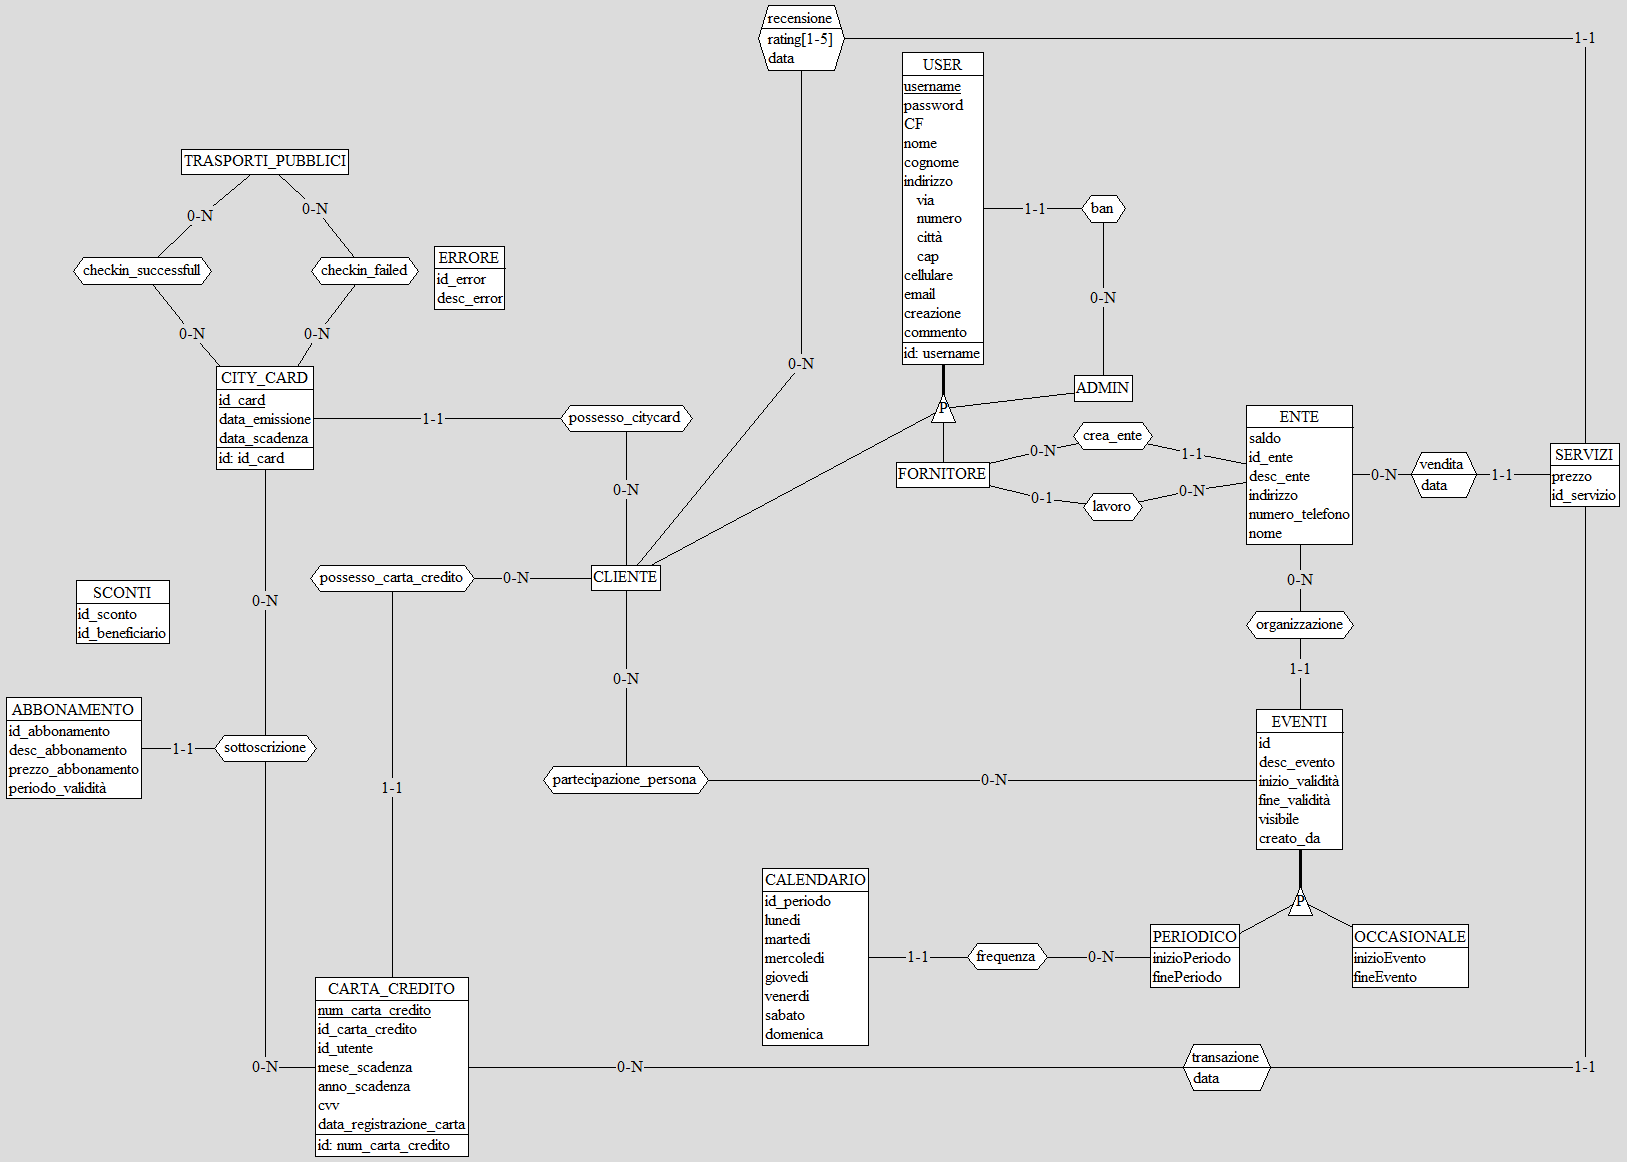
\includegraphics[width=0.9\paperwidth]{images/schema_ER_iniziale.png}}
\end{center}

\subsubsection{User}
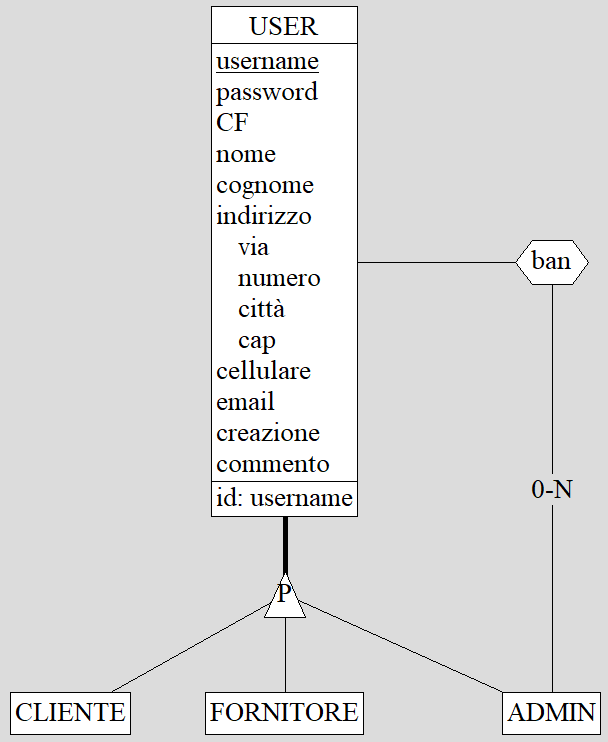
\includegraphics[width=0.95\columnwidth]{User.png}\\
I tre tipi di account che potranno essere creati, \textbf{CLIENTE}, \textbf{FORNITORE}, \textbf{ADMIN},  saranno sottocategorie di \textbf{USER}. Data la possibilità che una persona crei più di un account, ad esempio un fornitore vuole anche essere anche un cliente, l'identificazione avverrà tramite \textbf{username} e non il \textbf{CF}(codice fiscale).

\subsubsection{Ente}
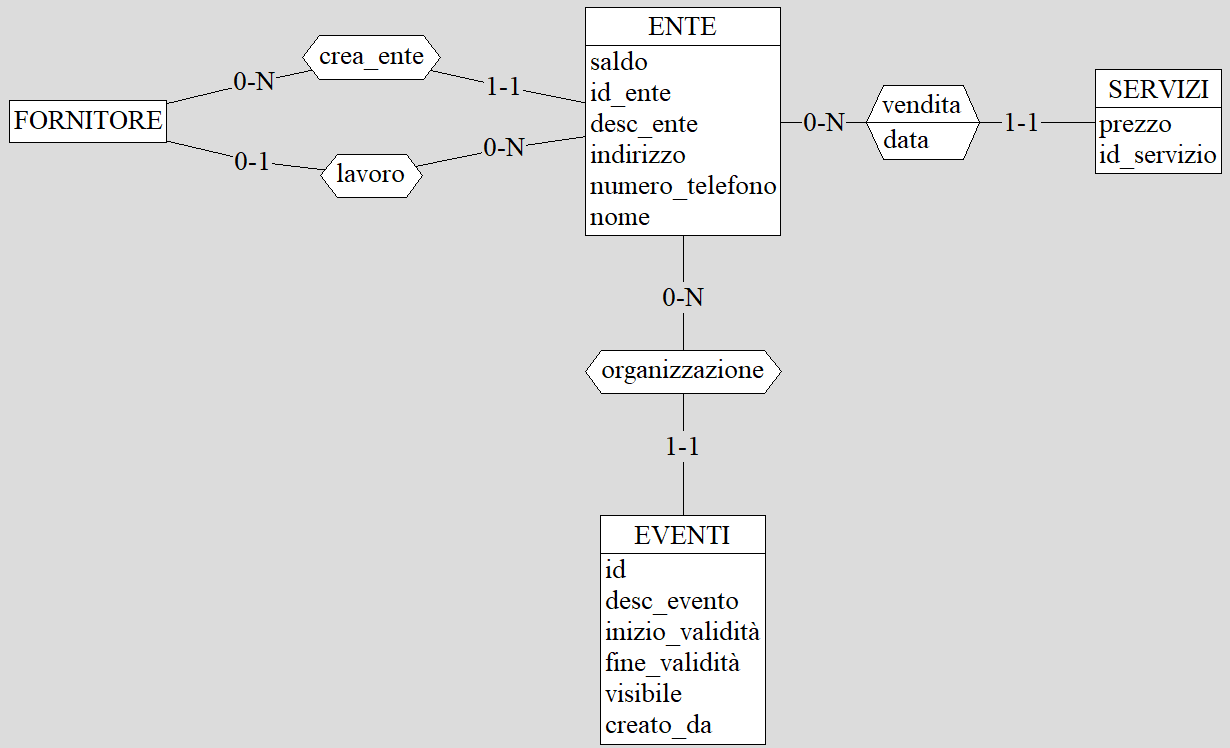
\includegraphics[width=0.95\columnwidth]{images/Ente.png} \\
L'ente è l'organizzazione che vende i servizi e organizza gli eventi. Possono venire creati dai fornitori. 
I fornitori possono associarsi ad un solo ente.


\subsubsection{Eventi}
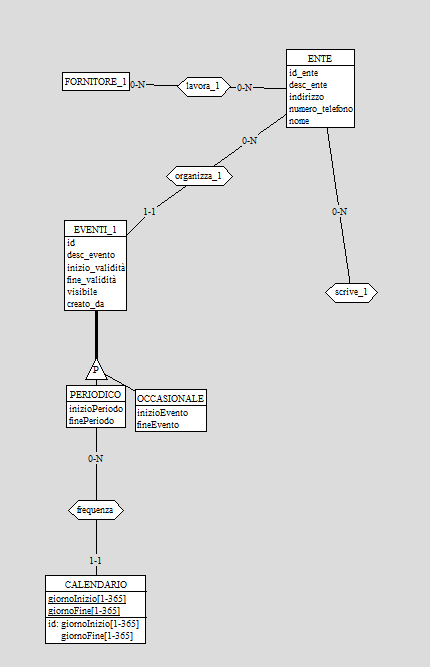
\includegraphics[width=0.95\columnwidth]{images/Eventi.png} \\
Gli eventi sono gli avvenimenti gratuiti accessibili dai clienti con prenotazione.
Sono organizzati dagli enti, un ente può organizzare più eventi ma un evento appartiene ad un solo ente.
Un evento può accadere in modalità periodica (ad esempio eventi a tema natalizio) oppure in modo occasionale (ad esempio inaugurazione di una nuova gelateria in centro).


\subsubsection{Servizi}
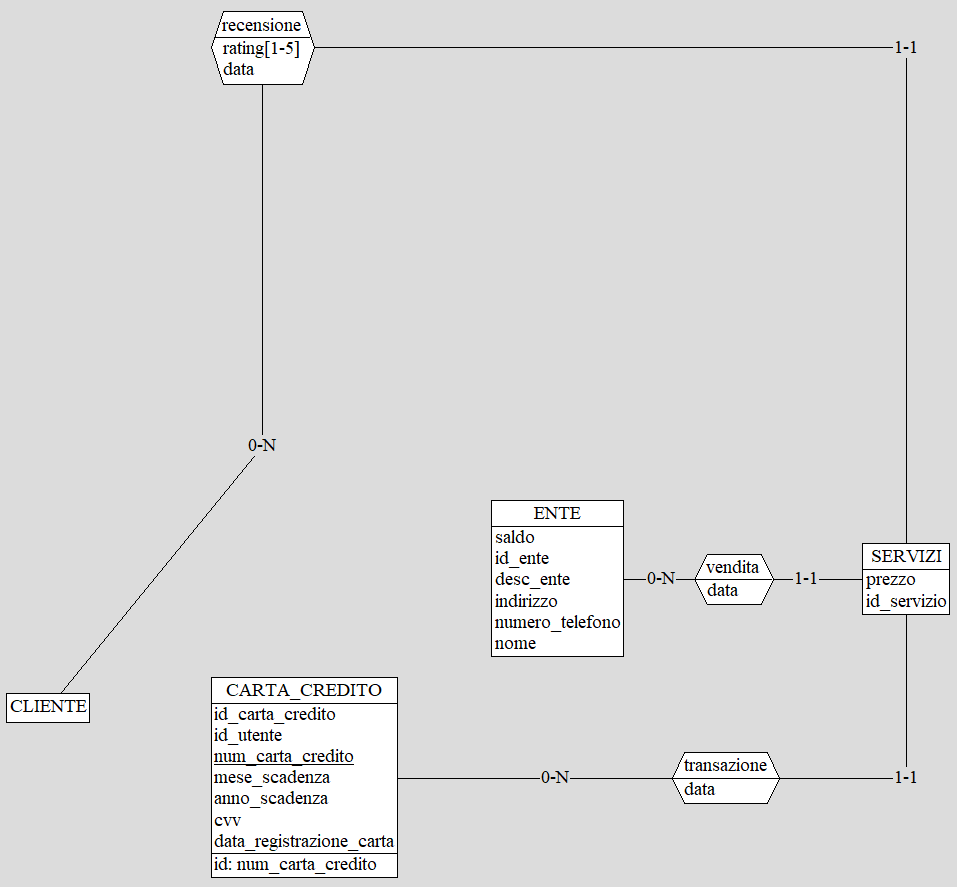
\includegraphics[width=0.95\columnwidth]{images/Servizi.png} \\
I servizi sono prodotti a pagamento accessibili dai clienti.
Sono venduti dagli enti, comprati tramite carta di credito e recensiti dai clienti dopo l'acquisto.


\subsubsection{CityCard}
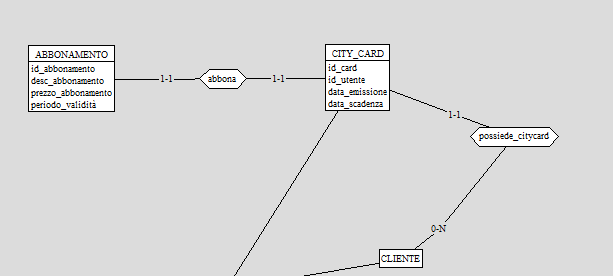
\includegraphics[width=0.95\columnwidth]{images/CityCard.png} \\
Ogni cliente può ottenere una CityCard che permetterà l'utilizzo gratuito dei mezzi pubblici e la prenotazione e l'acquisto di servizi forniti dagli enti. Per attivare la CityCard sarà necessario sottoscrivere ad un abbonamento a scelta tra tre diverse durate, dalla scelta fatta varierà la percentuale degli sconti applicati sui costi dei servizi.

\subsubsection{Trasporti Pubblici}
Si suppone che i trasporti pubblici siano una o più API esterne fornite dalla regione e/o da privati. Verrà creata una tabella con gli attributi minimali per imitarne la funzionalità. 


\subsubsection{Carta di credito}
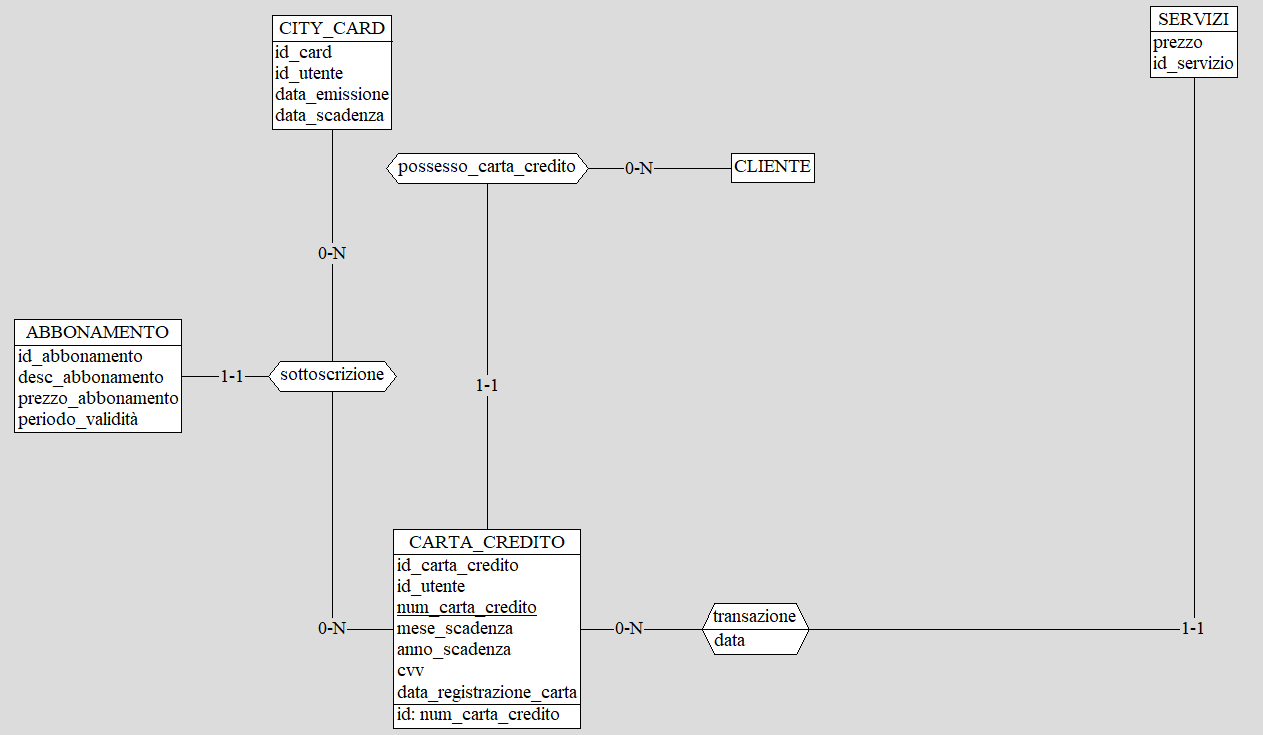
\includegraphics[width=0.95\columnwidth]{images/CartaDiCredito.png}\\
Ogni cliente, tramite la carta di credito, potrà acquistare l'abbonamento per la city card e pagare gli enti che forniscono i servizi.


\subsubsection{Abbonamento}
\includegraphics[width=0.95\columnwidth]{images/Abbonamento.png}\\
L'abbonamento è lo strumento che permette l'attivazione della city card e, di conseguenza, l'acquisto di servizi. Ogni abbonamento ha una sua fascia con prezzo, durata e percentuale di sconto diversi, l'utente potrà scegliere quale acquistare. A prescindere dalla tipologia ogni abbonamento ha un periodo di validità.

\subsubsection{Sconti}
Lo sconto si caratterizza per la percentuale di riduzione di prezzo applicata ai servizi.

\subsection{Schema scheletro prima delle correzioni}
\subsubsection{User}
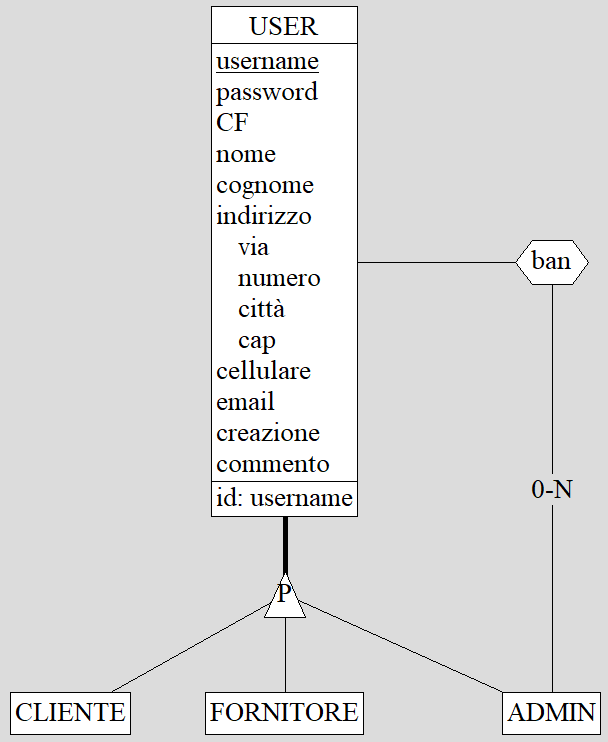
\includegraphics[width=0.95\columnwidth]{User.png}\\
I tre tipi di account che potranno essere creati, \textbf{CLIENTE}, \textbf{FORNITORE}, \textbf{ADMIN},  saranno sottocategorie di \textbf{USER}. Data la possibilità che una persona crei più di un account, ad esempio un fornitore vuole anche essere un cliente, l'identificazione avverrà tramite \textbf{username} e non il \textbf{CF}(codice fiscale).



\subsubsection{Ente}
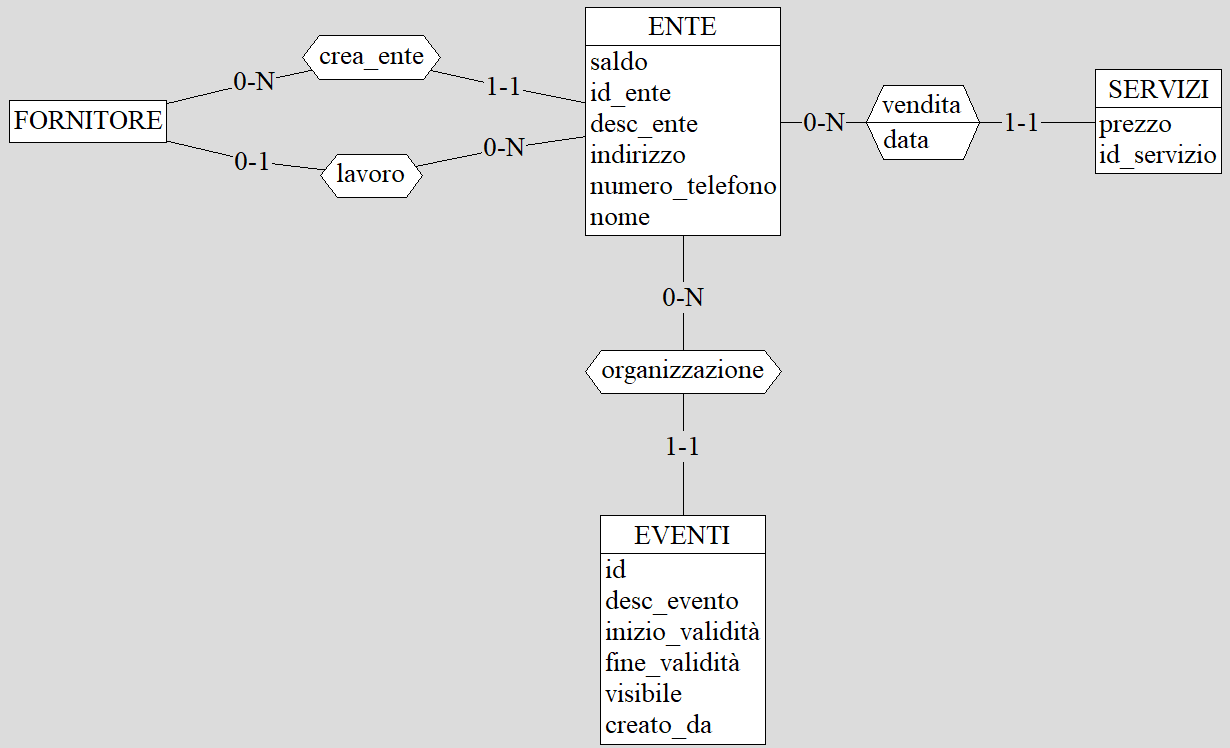
\includegraphics[width=0.95\columnwidth]{images/Ente.png} \\
L'ente è l'organizzazione che vende i servizi e organizza gli eventi. 
I fornitori possono lavorare per più di un ente.
Gli enti creano post e decidono quando pubblicarli/renderli pubblici. 


\subsubsection{Eventi}
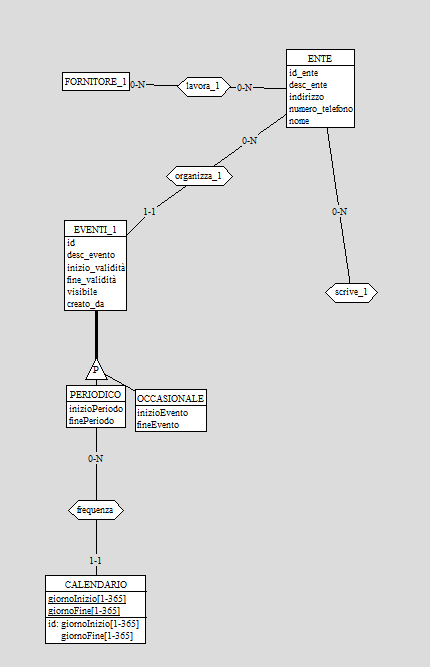
\includegraphics[width=0.95\columnwidth]{images/Eventi.png} \\
I servizi sono gli avvenimenti gratuito accessibili con o senza prenotazione.
Sono organizzati dagli enti, un ente può organizzare più eventi ma un evento appartiene ad un solo ente.
Un evento può accadere in modalità periodica (ad esempio eventi a tema natalizio) oppure in modo occasionale (ad esempio inaugurazione di una nuova gelateria in centro)
\subsubsection{CityCard}
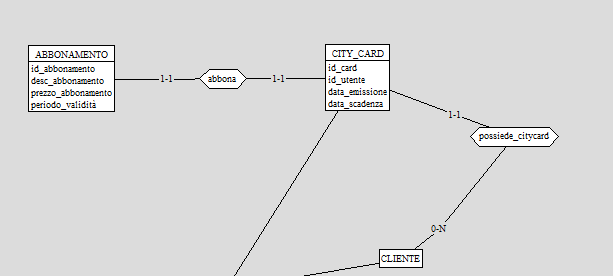
\includegraphics[width=0.95\columnwidth]{images/CityCard.png} \\
Ogni cliente può ottenere una CityCard che  permetterà l'utilizzo gratuito dei mezzi pubblici e la prenotazione e l'acquisto di servizi forniti dagli enti comunali e regionali. Per attivare la CityCard sarà necessario sottoscrivere ad un abbonamento a scelta tra tre diverse durate, dalla scelta fatta varierà la validità e gli sconti offerti  per l'acquisto dei servizi.
\subsubsection{Carta di credito} 
Ogni cliente, tramite la carta di credito, potrà acquistare la city card e pagare gli enti che forniscono i servizi
\subsubsection{Sezione delle news}
Una volta avuto accesso al portale ci sarà una sezione dedicata alle notizie relative ad eventi o servizi.
L'ente potrà creare un post in cui pubblicizza i servizi offerti o un'attività l'evento che sta organizzando
\subsubsection{Abbonamento}
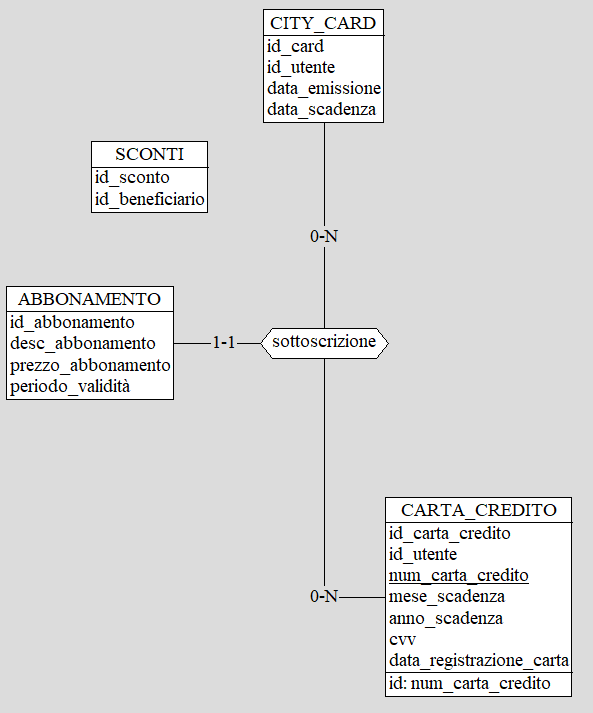
\includegraphics[width=0.95\columnwidth]{images/abbonamento.png}\\
L'abbonamento è lo strumento che permette l'attivazione della city card e, di conseguenza, l'acquisto di servizi. Ogni abbonamento ha una sua tipologia che l'utente potrà scegliere di acquistare. A prescindere dalla tipologia ogni abbonamento ha un suo prezzo e un periodo di validità.
\subsubsection{Sconti}
Lo sconto viene applicato in base ad alcune variabili: \\
    - età del cliente (se è sopra ai 65 anni di età) \\
    - se si è formato un gruppo si avrà una riduzione del servizio \\
Lo sconto si caratterizza per la percentuale di riduzione.

% \subsection{Schema concettuale finale} % TODO


\section{Progettazione Logica}

\subsection{Stima del volume dei dati}
Si fornisce in questa fase una tabella contenente il numero medio di istanze di ogni entità e associazione dello schema globale. \\

\begingroup % localize the following settings  
\setlength{\arrayrulewidth}{0.5mm}
\renewcommand{\arraystretch}{1.5}

\begin{longtblr}
[
  caption = {Stima del volume di dati},
  label = {tab:Stima del volume di dati},
]{
  colspec = {|X[3,l]X[2]X[2]X[6,l]|},
  rowhead = 1,
  hlines,
  row{even} = {lightgray},
  row{1} = {ColdPurple},
} 
Concetto & Costrutto & Volume & Descrizione\\
Utente & Entità & \num{100000} & Si stima che i clienti, gli enti e gli amministratori siano numerosi \\
Possiede CityCard & Relazione & \num{100000} & I clienti potrebbero registrarsi ma non avere una CityCard attiva e alcuni potrebbero avere più di una CityCard \\
Admin & Entità & \num{20} & Si stima che ci saranno 20 amministratori \\
Ente & Entità & \num{300} & Fornisce i servizi che il cliente usufruisce\\
Crea ente & Relazione & \num{300} & Ogni ente è creato da un fornitore \\
Fornitore & Entità & \num{800} & Si stima che ci siano 2-3 fornitori per ogni ente \\
Lavora & Relazione & \num{750} & Non tutti i fornitori lavorano per un ente \\
Servizi & Entità & \num{2400} & Data la cardinalità mi aspetto una stima di 8 servizi ad ente durante l'anno \\
Transazione & Relazione & \num{500000} & Si stima che in media ogni utente compri 5 servizi \\
Abbonamento & Entità & \num{3} & In ogni momento ci saranno 3 tipi di abbonamento\\
Sottoscrizione & Relazione & \num{100000} & Si stima una media di un abbonamento per ogni utente \\
Carta di credito & Entità & \num{150000} & Si stima che per ogni cliente sia associata più una carta di credito\\
Evento & Entità & \num{1200} & Si stima che vengano organizzati almeno 4 eventi per ente \\
Organizzazione evento & Relazione & \num{1200} & Essendo cardinalità 1-1 per ogni evento è prevista un'organizzazione\\
Partecipazione & Relazione & \num{30000} & Non tutti i clienti possono essere interessati agli eventi \\
Recensione & Relazione & \num{60000} & Ogni cliente può lasciare una recensione per servizio acquistato ma non è detto che tutti i clienti lo facciano \\
Sconto & Entità &  \num{6} & In base al periodo di alta o bassa stagione ci saranno sconti diversi \\
Riduzione & Relazione &  \num{3} & In ogni momento ci sarà uno sconto per ogni abbonamento\\
Ban & Relazione &  \num{100} & Si stima che ci saranno pochissimi utenti bannati \\
Frequenza & Relazione &  \num{600} & Stimo almeno un evento periodico per ogni ente \\
Errore & Entità &  \num{10} & Si stimano circa una decina di errori possibili\\
Checkin completo & Relazione &  \num{2000000} & Si stimano 20 viaggi per abbonamento\\
Checkin fallito & Relazione &  \num{1000} & Si stimano pochi errori durante la fase di check-in \\
Trasporto pubblico & Entità & ? & Sono API esterne, ignoro il loro volume

\end{longtblr}
\endgroup

\subsection{Operazioni richieste e la loro frequenza}
In questa fase esponiamo le tabelle delle operazioni utilizzate per costituire una stima delle principali operazioni richieste dal sito. La stima è su base \ul{settimanale}.



\begingroup % localize the following settings  
\setlength{\arrayrulewidth}{0.5mm}
\renewcommand{\arraystretch}{1.5}

% I = Interattiva
% B = Batch

\begin{longtblr}
[
  caption = {Operazioni richieste da tutti gli User},
  label = {tab:Operazioni richieste da tutti gli User},
]{
  colspec = {|X[1]X[8,l]X[3]X[1]X[8,l]|},
  rowhead = 1,
  hlines,
  row{even} = {lightgray},
  row{1} = {ColdPurple},
} 
Cod & Nome Operazione & Freq & Tipo & Descrizione\\
u.1 & Registrarsi alla piattaforma & \num{2100} & I & Registrazione al sito\\ 
u.2 & Accedere tramite login & \num{7000} & I & Login dell'account \\ 
u.3 & Modificare i dati del proprio account & \num{2100} & I & Login dell'account 
\end{longtblr}



\begin{longtblr}
  [
    caption = {Operazioni richieste amministratore},
    label = {tab:Operazioni richieste amministratore},
  ]{
    colspec = {|X[1]X[8,l]X[3]X[1]X[8,l]|},
    rowhead = 1,
    hlines,
    row{even} = {lightgray},
    row{1} = {CornflowerBlue},
  } 
  Cod & Nome Operazione & Freq & Tipo & Descrizione\\
  a.1 & Consultare la lista degli enti & \num{350} & I & Può consultare la lista degli enti registrati \\
  a.2 & Bannare gli altri utenti & \num{5} & I & L'admin può interdire l'accesso alla piattaforma \\ 
  a.3 & Reset delle recensioni & \num{5} & I & Può cancellare le recensioni \\
  a.4 & Consultazione statistiche & \num{400} & B & Può consultare statistiche globali della piattaforma \\
  \end{longtblr}
  

  \begin{longtblr}
    [
      caption = {Operazioni richieste da Fornitore},
      label = {tab:Operazioni richieste da Fornitore},
    ]{
      colspec = {|X[1]X[8,l]X[3]X[1]X[8,l]|},
      rowhead = 1,
      hlines,
      row{even} = {lightgray},
      row{1} = {LightCoral},
    } 
    Cod & Nome Operazione & Freq & Tipo & Descrizione\\
    f.1 & Creare enti & \num{50} & I & Il fornitore crea enti, all'apertura della piattaforma ci può essere un picco di operazioni al giorno ma poi calerà drasticamente \\ 
    f.2 & Associarsi a un ente  & \num{50} & I & Il deve associarsi al suo ente, con un picco iniziale come la creazione enti \\ 
    f.3 & Creare servizi & \num{50} & I & Il fornitore va a creare servizi \\
    f.4 & Creare eventi occasionali & \num{20} & I & Il fornitore crea eventi \\ 
    f.5 & Creare eventi periodici & \num{5} & I & Il fornitore crea eventi \\ 
    f.6 & Consultare statistiche riguardo il proprio ente  & \num{4000} & B & Il fornitore va a consultare una tabella contenente i dati\\ 
    
    \end{longtblr}


\begin{longtblr}
[
  caption = {Operazioni richieste dai Clienti},
  label = {tab:Operazioni richieste da cliente},
]{
  colspec = {|X[1]X[8,l]X[3]X[1]X[8,l]|},
  rowhead = 1,
  hlines,
  row{even} = {lightgray},
  row{1} = {ColdPurple},
} 
Cod & Nome Operazione & Freq & Tipo & Descrizione\\
c.1 & Richiedere una CityCard & \num{2000} & I & Il cliente può richiedere una CityCard \\ 
c.2 & Sottoscrivere un abbonamento & \num{2000} & I & Il cliente sottoscrive un abbonamento per utilizzare la piattaforma \\ 
c.3 & Aggiungere una carta di credito & \num{2000} & I & Il cliente memorizza una carta di credito nella piattaforma \\ 
c.4 & Rendere una carta di credito predefinita & \num{2000} & I & Il cliente rende predefinita la carta che utilizzera per gli acquisti \\ 
c.5 & Acquistare un servizio & \num{10000} & I & Il cliente può acquistare un servizio \\ 
c.6 & Prenotare un evento & \num{600} & I & Chiede all'applicativo una disponibilità di eventi \\
c.7 & Effettuare un check-in & \num{40000} & I & Chiede all'applicativo una disponibilità di eventi \\ 
c.8 & Consultare la lista degli acquisti fatti & \num{20000} & B & Consulta una lista \\ 
c.9 & Lasciare una recensione riguardo un servizio acquistato & \num{1500} & I & Il cliente rilascia una votazione \\ 
c.9 & Visualizzare lista servizi & \num{30000} & I & Il cliente visualizza la lista dei servizi disponibili \\ 
c.9 & Visualizzare lista eventi & \num{2000} & I & Il cliente visualizza la lista degli eventi disponibili \\ 

\end{longtblr}



\endgroup

\subsection{Schemi di navigazione}
Dopo aver determinato il volume dei dati ed aver associato a ciascuna operazione principale richiesta la frequenza di esecuzione procediamo ad esaminare gli schemi di navigazione per le principali operazioni richieste.

\subsubsection*{u.1 Registrazione di un nuovo utente}
L'utente si registra inserendo i dati minimi richiesti, in seguito potrà aggiungere altri campi modificando il proprio profilo.
\begin{longtblr}
[
  caption = {Registrazione di un nuovo utente},
]{
  colspec = {|X[3]X[1]X[2]X[4]|},
  rowhead = 1,
  hlines,
  row{even} = {PaleTurquoise},
  row{1} = {SkyBlue},
} 
Concetto & Costrutto & Accessi & Tipo\\
Users & E & 1 & Scrittura \\
\SetCell[c=4]{l, white} {
  Totale: 1S \textrightarrow 300/giorno\\
  Costo totale: 300 x (1\thinspace x \thinspace 2) = 600/giorno
  }

\end{longtblr}


\subsubsection*{u2. Login di un utente}
Per consentire il login si controlla che la combinazione username/password sia corretta e che l'utente non sia bannato. 
\begin{longtblr}
[
  caption = {Login di un utente},
]{
  colspec = {|X[3]X[1]X[2]X[4]|},
  rowhead = 1,
  hlines,
  row{even} = {PaleTurquoise},
  row{1} = {SkyBlue},
} 
Concetto & Costrutto & Accessi & Tipo\\
Users & E & 1 & L\\ 
\SetCell[c=4]{l, white} {
  Totale: 1L \textrightarrow 1500/giorno\\
  Costo totale: 1500 x (1) = 1500/giorno
  }

\end{longtblr}

\subsubsection*{u3. Modificare i dati del proprio account}
L'utente modifica i propri dati oppure inserisce quelli mancanti.
\begin{longtblr}
  [
    caption = {Modificare i dati del proprio account},
  ]{
    colspec = {|X[3]X[1]X[2]X[4]|},
    rowhead = 1,
    hlines,
    row{even} = {PaleTurquoise},
    row{1} = {SkyBlue},
  } 
  Concetto & Costrutto & Accessi & Tipo\\
  Users & E & 1 & S\\ 
  \SetCell[c=4]{l, white} {
  Totale: 1S \textrightarrow 300/giorno\\
  Costo totale: 300 x (1 \thinspace x \thinspace 2) = 600/giorno
  }
  \end{longtblr}

%%%%%%%%%%%%%%%%%%%%
%%%%%% ADMIN %%%%%%%
%%%%%%%%%%%%%%%%%%%%
\subsubsection*{a1. Consultare la lista degli utenti}
L'amministratore può visualizzare gli utenti registrati e bannarli o riattivarli all'occorrenza.
\begin{longtblr}
  [
    caption = {Consultare la lista degli utenti},
  ]{
    colspec = {|X[3]X[1]X[2]X[4]|},
    rowhead = 1,
    hlines,
    row{even} = {lightgray},
    row{1} = {LightCoral},
  } 
  Concetto & Costrutto & Accessi & Tipo\\
  User & E & 1 & L\\  
  ban & R & 1 & L\\ 
  \SetCell[c=4]{l, white} {
    Totale: 2L \textrightarrow 50/giorno\\
    Costo totale: 50 x (2) = 100/giorno
    }

  \end{longtblr}


  \subsubsection*{a2. Bannare gli altri utenti}
  Un amministratore banna un utente impedendone i futuri login.
  \begin{longtblr}
    [
      caption = {Bannare gli altri utenti},
    ]{
      colspec = {|X[3]X[1]X[2]X[4]|},
      rowhead = 1,
      hlines,
      row{even} = {lightgray},
      row{1} = {LightCoral},
    } 
    Concetto & Costrutto & Accessi & Tipo\\
    User & E & 1 & L\\
    ban & R & 1 & S \\ 

    \SetCell[c=4]{l, white} {
      Totale: 1L + 1S \textrightarrow 5/giorno\\
      Costo totale: 5 x (1 \thinspace + \thinspace 1 \thinspace x \thinspace 2) = 15/giorno
      }
  \end{longtblr}


\subsubsection*{a3. Reset delle recensioni}
In caso di necessità è possibile cancellare tutte le recensioni di un ente.
\begin{longtblr}
[
caption = {Reset delle recensioni},
]{
colspec = {|X[3]X[1]X[2]X[4]|},
rowhead = 1,
hlines,
row{even} = {lightgray},
row{1} = {LightCoral},
} 
Concetto & Costrutto & Accessi & Tipo\\
Ente & E & 1 & L \\
vendita & R & 1 & L \\
Servizio & E & 8 & L\\ 
Servizio & E & 8 & S\\ 
Recensione & R & 1600 (200 x 8) & L \\
Recensione & R & 1600 & S \\

\SetCell[c=4]{l, white} {
    Totale: 1610L + 1608S \textrightarrow 1/giorno\\
    Costo totale: 1 x (1610 \thinspace + \thinspace 1608 \thinspace x \thinspace 2) = \num{4826}/giorno
    }
\end{longtblr}



\subsubsection*{a4. Consultare le statistiche}
Verranno eseguite le query necessarie per ottenere le seguenti statistiche:\\
\begin{itemize}
  \item numero check-in
  \item numero check-in falliti
  \item numero CityCard attive
  \item numero eventi attivi
  \item numero servizi attivi
\end{itemize}
\begin{longtblr}
[
caption = {Consultare statistiche},
]{
colspec = {|X[3]X[1]X[2]X[4]|},
rowhead = 1,
hlines,
row{even} = {lightgray},
row{1} = {LightCoral},
} 
Concetto & Costrutto & Accessi & Tipo\\
checkin{\_}completato & R & 1 & L \\
checkin{\_}falliti & R & 2 & L \\
possesso{\_}CityCard & R & 1 & L \\
vendita & R & 1 & L \\
organizzazione & R & 1 & L \\

\SetCell[c=4]{l, white} {
    Totale: 5L \textrightarrow 50/giorno\\
    Costo totale: 50 x (5) = 250/giorno
    }
\end{longtblr}


%%%%%%%%%%%%%%%%%%%%%%%%
%%%%%% FORNITORE %%%%%%%
%%%%%%%%%%%%%%%%%%%%%%%%

\subsubsection*{f1. Creare enti}
Ogni fornitore può creare uno o più enti.
\begin{longtblr}
[
caption = {Creare enti},
]{
colspec = {|X[3]X[1]X[2]X[4]|},
rowhead = 1,
hlines,
row{even} = {lightgray},
row{1} = {ColdPurple},
} 
Ente & E & 1 & S \\
crea{\_}ente & R & 1 & S \\
\SetCell[c=4]{l, white} {
Totale: 2S \textrightarrow 8/giorno\\
Costo totale: 8 x (2 \thinspace x \thinspace 2) = 32/giorno
}
\end{longtblr}


\subsubsection*{f2. Associarsi a un ente}
Il fornitore si può associare a un solo ente.
\begin{longtblr}
[
caption = {Associarsi a un ente},
]{
colspec = {|X[3]X[1]X[2]X[4]|},
rowhead = 1,
hlines,
row{even} = {lightgray},
row{1} = {ColdPurple},
} 
Concetto & Costrutto & Accessi & Tipo\\
lavoro & R & 1 & S \\ 
\SetCell[c=4]{l, white} {
    Totale: 1S \textrightarrow 3/giorno\\
    Costo totale: 3 x (1 \thinspace x \thinspace 2) = 6/giorno
    }
\end{longtblr}

\subsubsection*{f3. Creare servizi}
Ogni fornitore associato ad un ente può creare servizi.
\begin{longtblr}
[
caption = {Creare servizi},
]{
colspec = {|X[3]X[1]X[2]X[4]|},
rowhead = 1,
hlines,
row{even} = {lightgray},
row{1} = {ColdPurple},
} 
Concetto & Costrutto & Accessi & Tipo\\
vendita & R & 1 & S \\
Servizio & E & 1 & S \\
lavoro & R & 1 & L \\
\SetCell[c=4]{l, white} {
    Totale: 1L + 1S \textrightarrow 10/giorno\\
    Costo totale: 10 x (1 \thinspace + \thinspace 2 \thinspace x \thinspace 2) = 50/giorno
    }
\end{longtblr}


\subsubsection*{f4. Creare eventi occasionali}
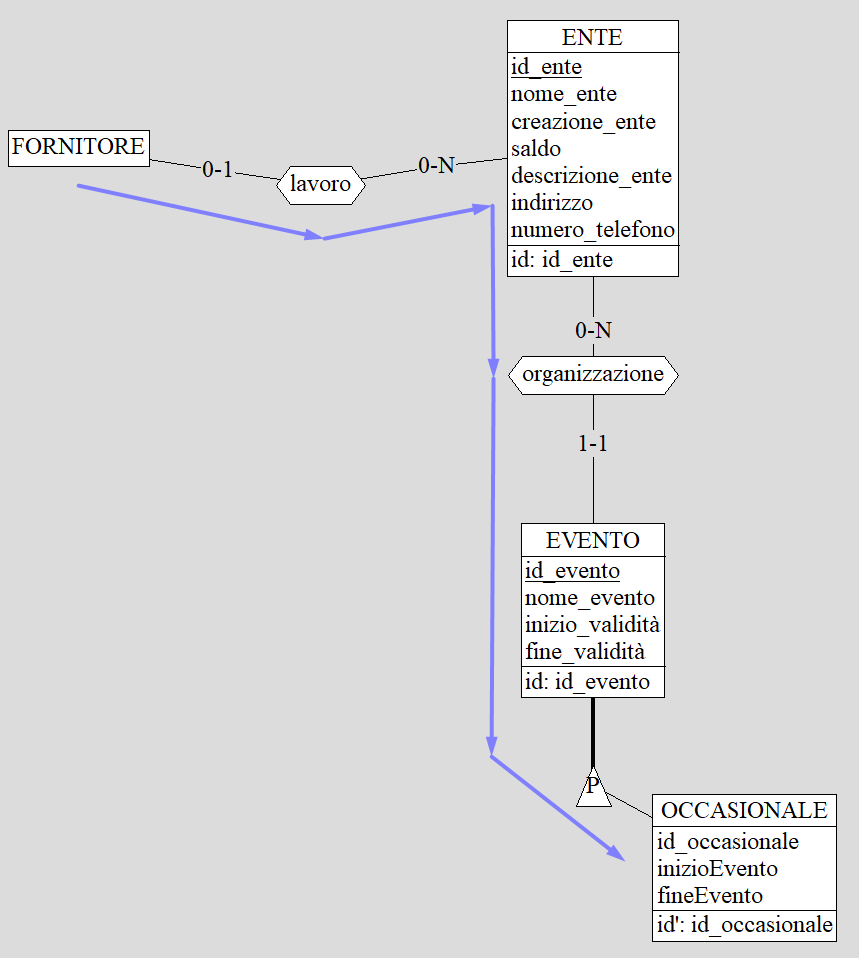
\includegraphics[width=0.95\columnwidth]{f4creaEventoOccasionale.png}\\
I fornitori associati a un ente possono creare eventi occasionali.
\begin{longtblr}
[
caption = {Creare eventi occasionali},
]{
colspec = {|X[3]X[1]X[2]X[4]|},
rowhead = 1,
hlines,
row{even} = {lightgray},
row{1} = {ColdPurple},
} 
Concetto & Costrutto & Accessi & Tipo\\
lavoro & R & 1 & L \\
organizza & R & 1 & S \\
Evento & E & 1 & S \\
Occasionale & E & 1 & S \\
\SetCell[c=4]{l, white} {
    Totale: 1L + 3S \textrightarrow 4/giorno\\
    Costo totale: 4 x (1 \thinspace + \thinspace 3 \thinspace x \thinspace 2) = 28/giorno
    }
\end{longtblr}




\subsubsection*{f5. Creare eventi periodici}
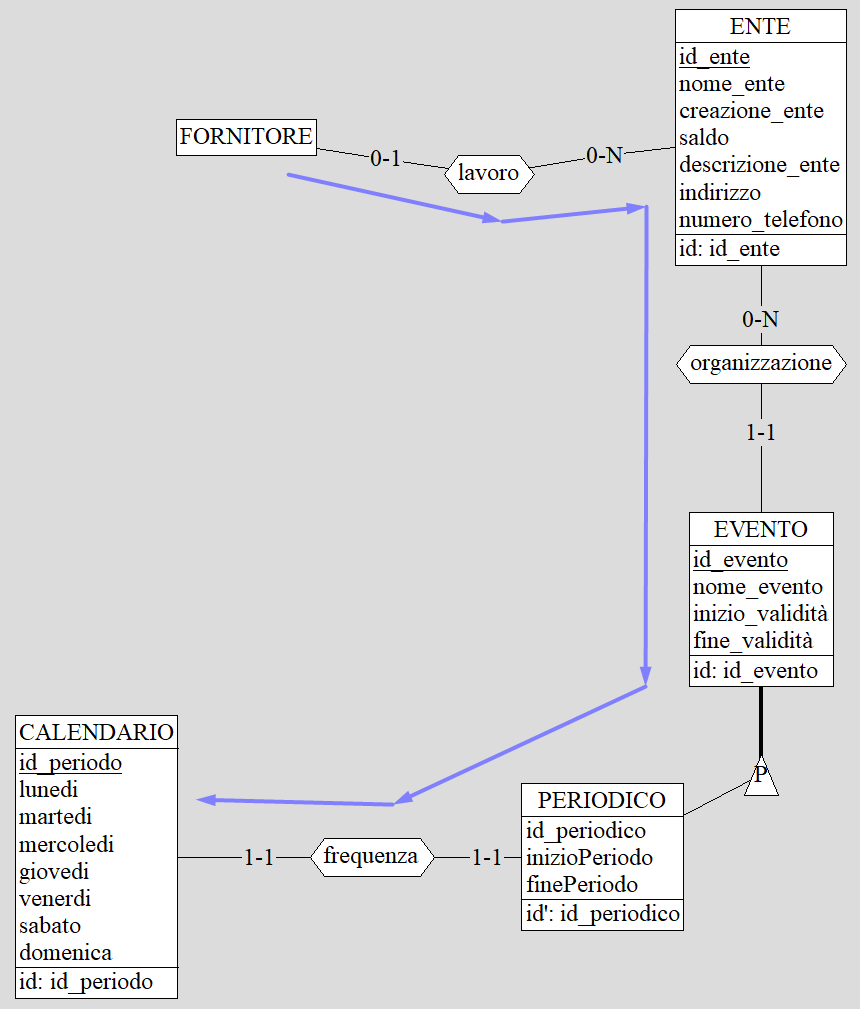
\includegraphics[width=0.95\columnwidth]{f5creaEventoPeriodico.png}\\
Per creare un evento periodico si dovrà ottenere l'id dell'ente al quale è associato il fornitore, poi andare a creare un record per l'evento e un altro record per il periodo. \\
\begin{longtblr}
[
caption = {Creare eventi periodici},
]{
colspec = {|X[3]X[1]X[2]X[4]|},
rowhead = 1,
hlines,
row{even} = {lightgray},
row{1} = {ColdPurple},
} 
Concetto & Costrutto & Accessi & Tipo\\
lavoro & R & 1 & L \\
organizza & R & 1 & S \\
Evento & E & 1 & S \\
Periodico & E & 1 & L \\
frequenza & R & 1 & S \\
Calendario & E & 1 & S \\
\SetCell[c=4]{l, white} {
    Totale: 2L + 4S \textrightarrow 1/giorno\\
    Costo totale: 1 x (2 \thinspace + \thinspace 4 \thinspace x \thinspace 2) = 10/giorno
    }
\end{longtblr}



\subsubsection*{f6. Consultare statistiche riguardo il proprio ente}
Oltre alla query per ottenere l'id dell'ente del fornitore verranno eseguite quelle necessarie per ottenere le seguenti statistiche:\\
\begin{itemize}
  \item saldo dell'ente associato al fornitore
  \item numero eventi attivi
  \item numero servizi attivi
\end{itemize}

\begin{longtblr}
[
caption = {Consultare statistiche riguardo il proprio ente},
]{
colspec = {|X[3]X[1]X[2]X[4]|},
rowhead = 1,
hlines,
row{even} = {lightgray},
row{1} = {ColdPurple},
} 
Concetto & Costrutto & Accessi & Tipo\\
Ente & E & 1 & L \\
Eventi & E & 1 & L\\ 
Servizi & E & 1 & L\\ 
\SetCell[c=4]{l, white} {
    Totale: 2L \textrightarrow 800/giorno\\
    Costo totale: 800 x (3) = 2400/giorno
    }
\end{longtblr}

%%%%%%%%%%%%%%%%%%%%%%
%%%%%% CLIENTE %%%%%%%
%%%%%%%%%%%%%%%%%%%%%%
\subsubsection*{c1. Richiedere una CityCard}
Il cliente richiede una nuova CityCard.
\begin{longtblr}
[
caption = {Richiedere una CityCard},
]{
colspec = {|X[3]X[1]X[2]X[4]|},
rowhead = 1,
hlines,
row{even} = {lightgray},
row{1} = {MediumSeaGreen},
} 
Concetto & Costrutto & Accessi & Tipo \\
possesso{\_}cityCard & R & 1 & S \\
CityCard & E & 1 & S \\
\SetCell[c=4]{l, white} {
    Totale: 2S \textrightarrow 2000/giorno\\
    Costo totale: 2000 x (2 \thinspace x \thinspace 2) = 8000/giorno
    }
\end{longtblr}

\subsubsection*{c2. Sottoscrivere un abbonamento}
Prima di sottoscrivere un abbonamento vengono cercate una CityCard valida e una carta di credito predefinita. \\
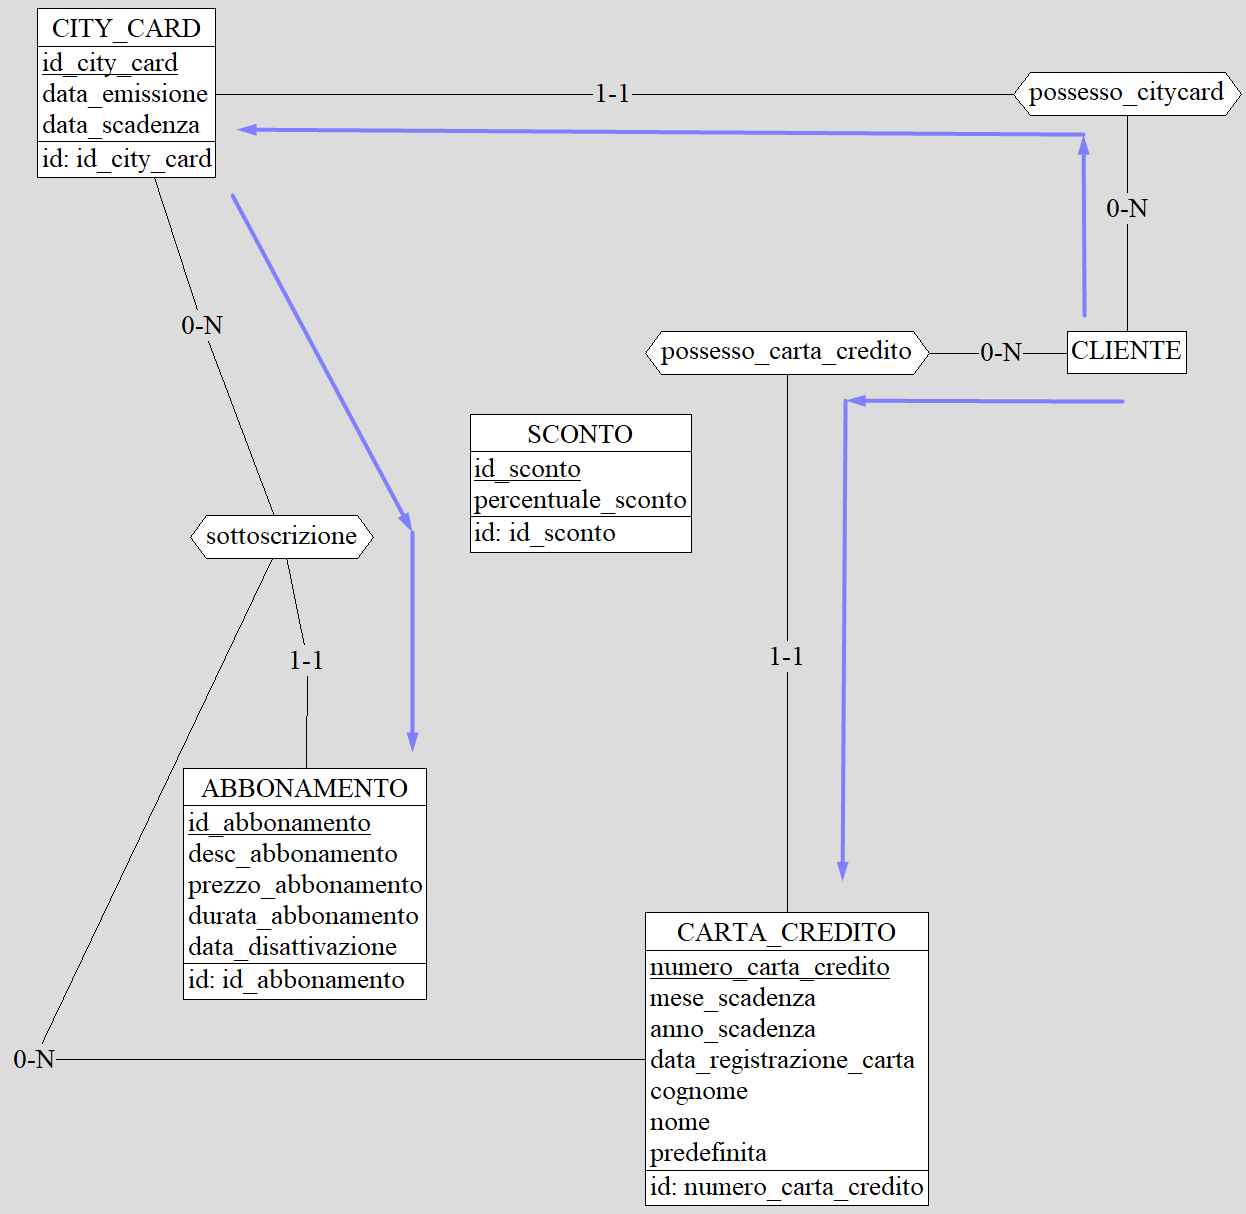
\includegraphics[width=0.95\columnwidth]{c2sottoscrizioneAbbonamento.png}\\

\begin{longtblr}
[
caption = {Sottoscrivere un abbonamento},
]{
colspec = {|X[3]X[1]X[2]X[4]|},
rowhead = 1,
hlines,
row{even} = {lightgray},
row{1} = {MediumSeaGreen},
} 
Concetto & Costrutto & Accessi & Tipo \\
Cliente & E & 1 & L\\ 
possesso{\_}carta{\_}credito & R & 1 & L \\
Carta{\_}Credito & E & 1 & L \\
possesso{\_}citycard & R & 1 & L \\
CityCard & E & 1 & L \\
sottoscrizione & R & 1 & S \\
\SetCell[c=4]{l, white} {
    Totale: 5L + 1S \textrightarrow 2000/giorno\\
    Costo totale: 2000 x (5 \thinspace + \thinspace 1 \thinspace x \thinspace 2) = 16000/giorno
    }
\end{longtblr}


\subsubsection*{c3. Aggiungere una carta di credito}
Un cliente può salvare le proprie carte di credito.
\begin{longtblr}
[
caption = {Aggiungere una carta di credito},
]{
colspec = {|X[3]X[1]X[2]X[4]|},
rowhead = 1,
hlines,
row{even} = {lightgray},
row{1} = {MediumSeaGreen},
} 
Concetto & Costrutto & Accessi & Tipo \\
Carta{\_}credito & R & S \\
possesso{\_}carta{\_}credito & R & 1 & S \\
\SetCell[c=4]{l, white} {
    Totale: 2S \textrightarrow 2000/giorno\\
    Costo totale: 2000 x (2 \thinspace x \thinspace 2) = 8000/giorno
    }
\end{longtblr}


\subsubsection*{c4. Rendere una carta di credito predefinita}
Rendo predefinita una carta di credito di un utente e non predefinite tutte le altre.\\
(dato che in media ho 1,5 carte per cliente, approssimo a 2)
\begin{longtblr}
[
caption = {Aggiungere una carta di credito},
]{
colspec = {|X[3]X[1]X[2]X[4]|},
rowhead = 1,
hlines,
row{even} = {lightgray},
row{1} = {MediumSeaGreen},
} 
Concetto & Costrutto & Accessi & Tipo \\
possesso{\_}carta{\_}credito & R & 2 & L \\
Carta{\_}credito & R & 2 & L \\
Carta{\_}credito & R & 2 & S \\
\SetCell[c=4]{l, white} {
    Totale: 4L + 2S \textrightarrow 2000/giorno\\
    Costo totale: 2000 x (4 \thinspace + \thinspace 2 \thinspace x \thinspace 2) = 16000/giorno
    }
\end{longtblr}


\subsubsection*{c5. Acquistare un servizio}
Viene controllata la CityCard dell'utente, tramite essa vengono recuperati i dati della sottoscrizione, poi quelli dello sconto, con questi dati viene calcolato il prezzo e infine viene comprato il servizio e aggiornato il saldo dell'ente.
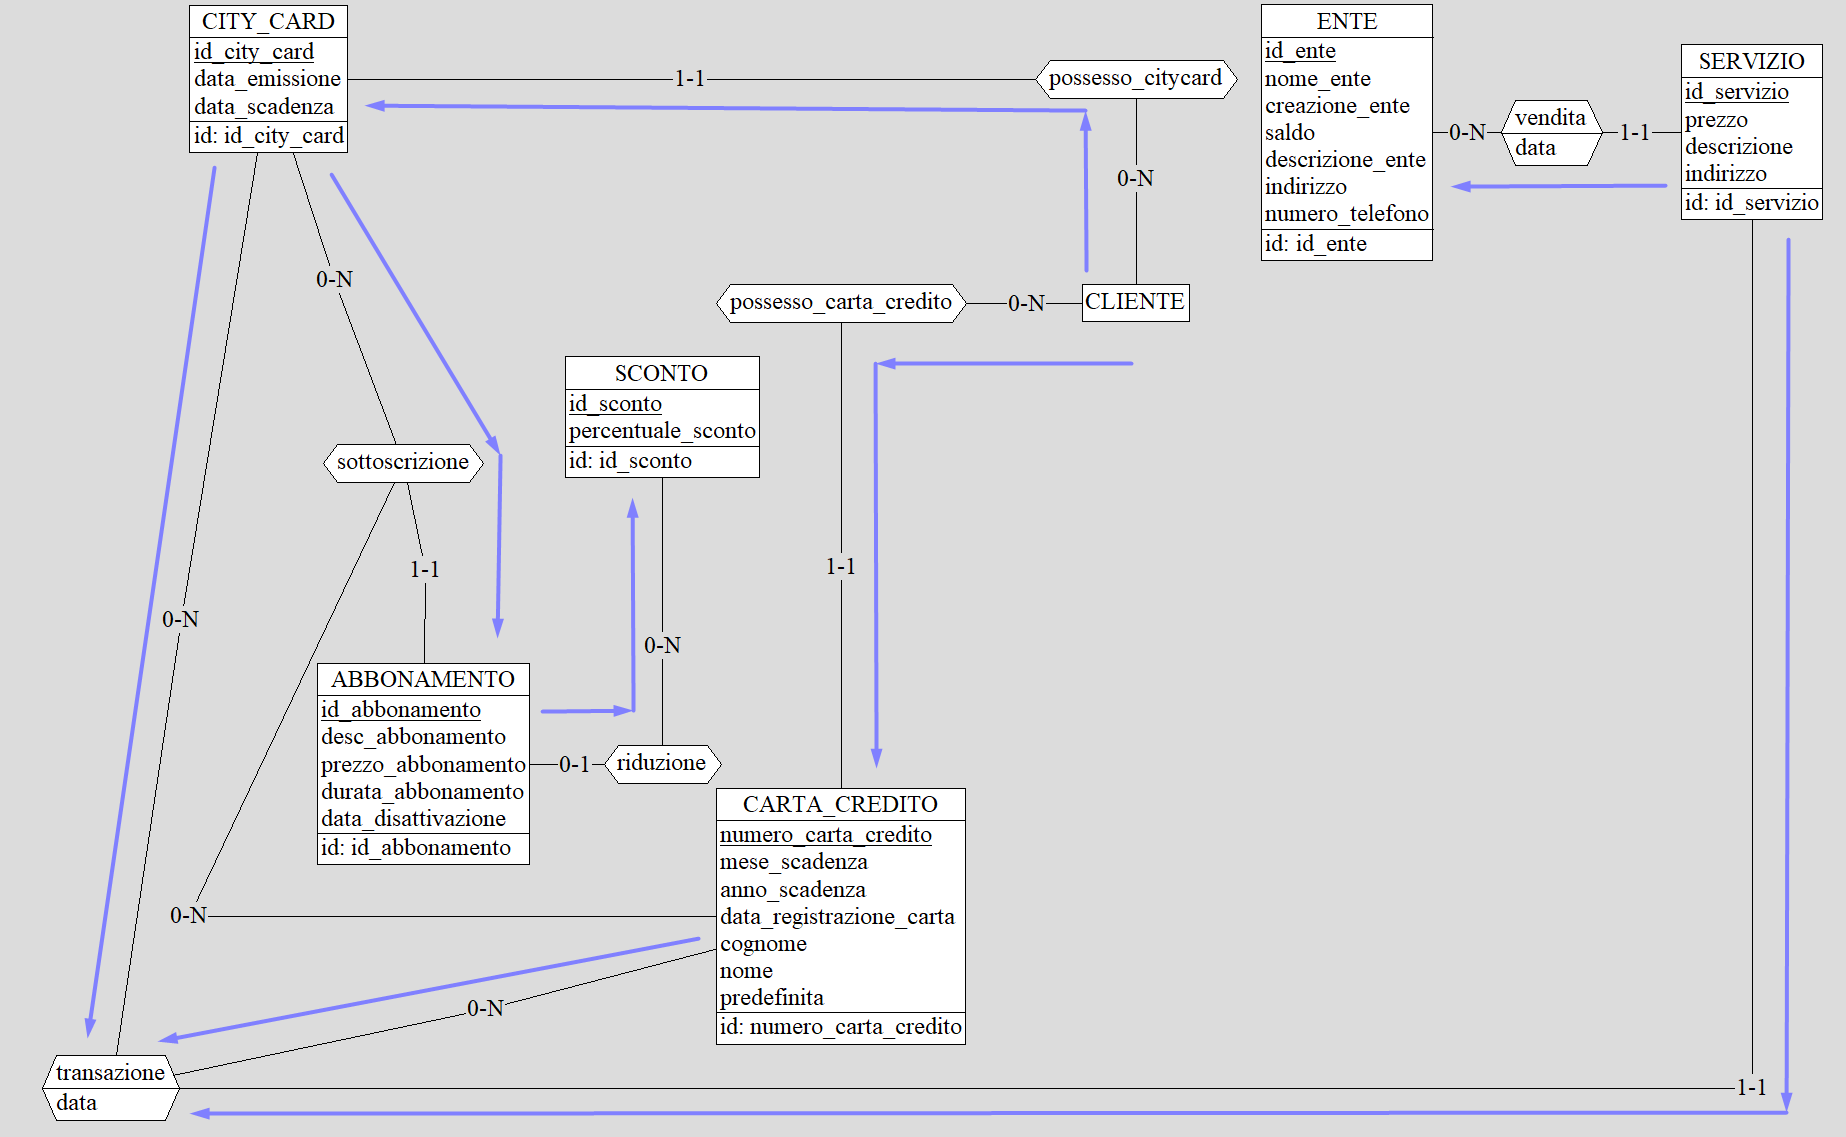
\includegraphics[width=0.95\columnwidth]{c5acquistaServizio.png}\\

\begin{longtblr}
[
caption = {Acquistare un servizio},
]{
colspec = {|X[3]X[1]X[2]X[4]|},
rowhead = 1,
hlines,
row{even} = {lightgray},
row{1} = {MediumSeaGreen},
} 
Concetto & Costrutto & Accessi & Tipo \\
possesso{\_}citycard & R & 1 & L \\
CityCard & E & 1 & L\\ 
sottoscrizione & R & 1 & L \\
Abbonamento & E & 1 & L\\ 
riduzione & R & 1 & L \\
Sconto & E & 1 & L\\ 
possesso{\_}carta{\_}credito & R & 1 & L \\
Carta{\_}credito & E & 1 & L \\
transazione & R & 1 & S\\ 
Servizio & E & 1 & L\\ 
vendita & R & 1 & L\\ 
Ente & E & 1 & S\\ 
\SetCell[c=4]{l, white} {
    Totale: 10L + 2S \textrightarrow 3000/giorno\\
    Costo totale: 3000 x (10 \thinspace + \thinspace 2 \thinspace x \thinspace 2) = 42000/giorno
    }
\end{longtblr}

\subsubsection*{c6. Prenotare un evento}
Gli utenti possono prenotare gratuitamente degli eventi.
\begin{longtblr}
[
caption = {Prenotare un evento},
]{
colspec = {|X[3]X[1]X[2]X[4]|},
rowhead = 1,
hlines,
row{even} = {lightgray},
row{1} = {MediumSeaGreen},
} 
Concetto & Costrutto & Accessi & Tipo \\
partecipazione{\_}persona & R & 1 & S \\
\SetCell[c=4]{l, white} {
    Totale: 1S \textrightarrow 500/giorno\\
    Costo totale: 500 x (1 \thinspace x \thinspace 2) = 1000/giorno
    }
\end{longtblr}


\subsubsection*{c7. Effettuare un check-in}
Per poter effettuare un check-in devo confermare che la CityCard del cliente sia valida.
\begin{longtblr}
[
caption = {Effettuare un check-in},
]{
colspec = {|X[3]X[1]X[2]X[4]|},
rowhead = 1,
hlines,
row{even} = {lightgray},
row{1} = {MediumSeaGreen},
} 
Concetto & Costrutto & Accessi & Tipo \\
possesso{\_}citycard & R & 1 & L \\
CityCard & E & 1 & L\\ 
checkin(completato/fallito) & R & 1 & S \\
\SetCell[c=4]{l, white} {
    Totale: 2L + 1S \textrightarrow 5000/giorno\\
    Costo totale: 5000 x (2 \thinspace + \thinspace 1 \thinspace x \thinspace 2) = 20000/giorno
    }
\end{longtblr}

\subsubsection*{c8. Consultare la lista degli acquisti fatti}
Un utente può visualizzare la lista di tutti gli acquisti fatti.
\begin{longtblr}
[
caption = {Consultare la lista degli acquisti fatti},
]{
colspec = {|X[3]X[1]X[2]X[4]|},
rowhead = 1,
hlines,
row{even} = {lightgray},
row{1} = {MediumSeaGreen},
} 
Concetto & Costrutto & Accessi & Tipo \\
possesso{\_}citycard & R & 1 & L \\
CityCard & E & 1 & L\\ 
transazione & R & 1 & L\\ 
\SetCell[c=4]{l, white} {
    Totale: 3L \textrightarrow 3000/giorno\\
    Costo totale: 3000 x (3) = 9000/giorno
    }
\end{longtblr}


\subsubsection*{c9. Lasciare una recensione riguardo un servizio acquistato}
Questa funzionalità verrà approfondita nella prossima sezione dedicata al calcolo delle ridondanze.

\subsubsection*{c10. Visualizzare lista servizi}
Anche questa funzionalità verrà approfondita nella prossima sezione dedicata al calcolo delle ridondanze.


\subsubsection*{c11. Visualizzare lista eventi}
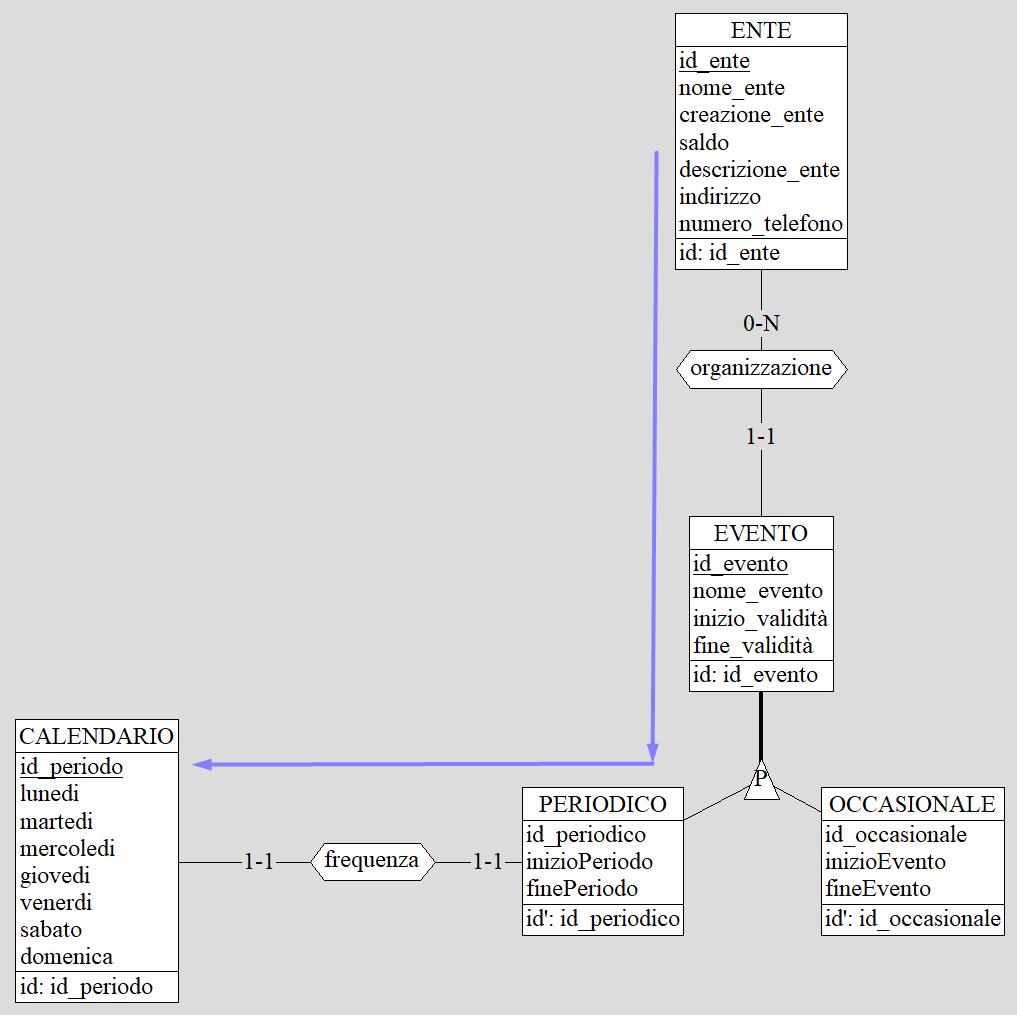
\includegraphics[width=0.95\columnwidth]{c11getEventi.png}\\
L'utente visualizza la lista di tutti gli eventi disponibili, sia periodici che occasionali.
\begin{longtblr}
[
caption = {Visualizzare lista eventi},
]{
colspec = {|X[3]X[1]X[2]X[4]|},
rowhead = 1,
hlines,
row{even} = {lightgray},
row{1} = {MediumSeaGreen},
} 
Concetto & Costrutto & Accessi & Tipo \\
Ente & E & 1 & L \\
organizzazione & R & 1 & L \\
Occasionale & E & 1 & L\\ 
Periodico & E & 1 & L\\ 
frequenza & R & 1 & L \\
Calendario & E & 1 & L\\ 

\SetCell[c=4]{l, white} {
    Totale: 6L \textrightarrow 1500/giorno\\
    Costo totale: 1500 x (6) = 9000/giorno
    }
\end{longtblr}


\subsection{Frequenza e costo degli accessi}

\subsection{Analisi delle ridondanze}
% TODO sostituire partecipanti con recensioni

In questa fase ci occuperemo dell'analisi delle ridondanze cioè quella informazioni che possono essere ricavate altrove.
Una ridondanza quindi corrisponde ad un dato che può essere derivato, cioè ottenuto attraverso una serie di operazioni, da altri dati.
Se si mantiene la ridondanza si semplificano alcune interrogazioni ma si occupa maggior spazio.
All'interno del nostro schema possiamo fare alcune considerazioni.

\begin{itemize}
    \item L'attributo numero{\_}partecipanti è derivabile da una operazione di conteggio delle istanze di clienti che hanno prenotato un evento.
    Dobbiamo tenere conto delle frequenze di esecuzione.
    \begin{itemize}
        \item operazione 1: si tiene il conteggio ogni volta che un cliente prenota un evento
        \item operazione 2: vengono visualizzati tutti i dati di un evento
    \end{itemize}
\end{itemize}

\subsection{Raffinamento dello schema} % TODO
\subsubsection{Nomenclatura tabelle}
Si è deciso di standardizzare i nomi di tutte le tabelle scegliendo sostantivi plurali.

\subsubsection{Eliminazione delle gerarchie di generalizzazione}
Nel processo di definizione del nostro schema concettuale, abbiamo identificato alcune gerarchie di generalizzazione che richiedevano un'analisi approfondita per determinare la loro utilità e struttura all'interno del modello. Dopo un'attenta valutazione, abbiamo deciso di semplificare queste gerarchie, adottando una strategia di riduzione che ha portato all'eliminazione delle generalizzazioni e alla fusione degli attributi dei sottotipi nelle entità principali. Di seguito, illustriamo le specifiche modifiche effettuate:

\begin{itemize} 
\item 
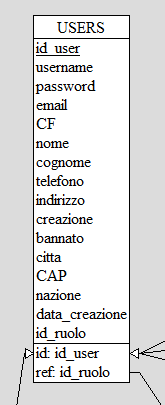
\includegraphics[width=0.95\columnwidth]{UserLogico.png}\\
Generalizzazione dell’entità \textit{User}: Inizialmente, l’entità \textit{User} era rappresentata come una generalizzazione totale ed esclusiva con tre sottotipi distinti: \textit{Cliente}, \textit{Admin} e \textit{Fornitore}. Tuttavia, durante la fase di progettazione, abbiamo riscontrato che tutti i sottotipi condividevano gli stessi attributi fondamentali, rendendo superflua la distinzione tra essi. Pertanto, abbiamo deciso di far collassare la gerarchia verso l’alto, integrando gli attributi direttamente nell’entità \textit{User}. Questo approccio ha semplificato la struttura del modello, migliorando la chiarezza e l'efficienza nella gestione dei dati senza perdere informazioni rilevanti.
\item 
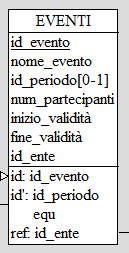
\includegraphics[width=0.95\columnwidth]{EventiLogico.png}\\
Generalizzazione dell’entità \textit{Eventi}: 
Analogamente, l’entità \textit{Eventi} era inizialmente strutturata come una generalizzazione totale ed esclusiva, comprendente i sottotipi \textit{Periodico} e \textit{Occasionale}, utilizzati per definire la natura dell'evento. Tuttavia, analizzando l’architettura del sistema, abbiamo ritenuto più efficiente eliminare la gerarchia e incorporare i sottotipi come attributi dell’entità principale \textit{Eventi}. Questa scelta ha permesso di mantenere la flessibilità nella classificazione degli eventi, riducendo al contempo la complessità del modello e facilitando la gestione delle informazioni relative agli eventi.
\end{itemize}

\subsubsection{Chiavi esterne}
Vengono utilizzate, per semplicità, chiavi esterne con lo stesso nome della chiave primaria a cui fanno riferimento.






\section{Traduzione delle entità}
\begin{itemize}
    \item 
    \textbf{Carta{\_}credito}(\underline{num{\_}carta{\_}credito}, cognome{\_}associato, nome{\_}associato,
    mese{\_}scadenza, anno{\_}scadenza, data{\_}registrazione{\_}carta, id{\_}user,
    predefinita)\\
    FK: id{\_}user \textrightarrow USERS.id{\_}user

    \item 
    \textbf{Checks}(\underline{id{\_}check}, 
    orario{\_}convalida,
    id{\_}city{\_}card,
    id{\_}mezzo,
    id{\_}stato)\\
    FK: id{\_}mezzo \textrightarrow MEZZI.id{\_}mezzo\\
    FK: id{\_}stato \textrightarrow STATI{\_}CHECK.id{\_}stato\\
    FK: id{\_}city{\_}card \textrightarrow CITY{\_}CARD.id{\_}city{\_}card\\

    \item 
    \textbf{CityCard}
    (\underline{id{\_}city{\_}card},
    id{\_}utente,
    data{\_}emissione,
    data scadenza)

    \item 
    \textbf{Collaborazioni}
    (\underline{id{\_}collaborazione},
    inizio{\_}collaborazione,
    fine{\_}collaborazione,
    id{\_}user,
    id{\_}ente)\\
    FK: id{\_}user \textrightarrow USER.id{\_}user\\
    FK: id{\_}ente \textrightarrow ENTI.id{\_}ente

    \item
    \textbf{Enti}
    (\underline{id{\_}ente}
    descrizione{\_}ente,
    saldo,
    indirizzo,
    numero{\_}telefono,
    nome,
    id{\_}user)\\
    FK: id{\_}user \textrightarrow USERS id{\_}user
    
    \item 
    \textbf{Eventi}
    (\underline{id{\_}evento},
    nome{\_}evento,
    num{\_}partecipanti,
    id{\_}periodo,
    inizio{\_}validità,
    fine{\_}validità,
    id{\_}ente)\\
    FK: id{\_}periodo \textrightarrow PERIODI.id{\_}periodo,\\
    FK: id{\_}ente \textrightarrow ENTI.id{\_}ente
    
    \item 
    \textbf{Listino abbonamenti}
    (\underline{id{\_}listino{\_}abbonamento},
    descrizione{\_}abbonamento,
    prezzo{\_}abbonamento,
    durata{\_}abbonamento,
    data{\_}disattivazione,
    id{\_}sconto)\\
    FK: id{\_}sconto \textrightarrow SCONTI.id{\_}sconto
    
    \item 
    \textbf{Mezzi}
    (\underline{id{\_}mezzo},
    desc{\_}mezzo,
    partenza,
    destinazione
    )

    \item 
    \textbf{Partecipazioni}
    (\underline{id{\_}partecipazione},
    data{\_}registrazione,
    id{\_}evento,
    id{\_}city{\_}card)\\
    FK: id{\_}city{\_}card \textrightarrow CITY{\_}CARD.id{\_}city{\_}card,\\
    FK: id{\_}evento \textrightarrow EVENTI.id{\_}evento

    \item   
    \textbf{Periodi}
    (\underline{id{\_}periodo},
    lunedi,
    martedi,
    mercoledi,
    giovedi,
    venerdi,
    sabato,
    domenica)

    \item 
    \textbf{Recensioni}
    (\underline{id{\_}recensione},
    data{\_}inserimento,
    votazione,
    id{\_}servizio,
    id{\_}user)\\
    FK: id{\_}servizio \textrightarrow SERVIZI.id{\_}servizio,\\
    FK: id{\_}user \textrightarrow USERS.id{\_}user

    \item 
    \textbf{Ruoli}
    (\underline{id{\_}ruolo},
    descrizione{\_}ruolo
    )

    \item 
    \textbf{Sconti}
    (\underline{id{\_}sconto},
    percentuale{\_}sconto)

    \item 
    \textbf{Servizi}
    (\underline{id{\_}servizio},
    prezzo,
    data{\_}inserimento,
    data{\_}termine,
    descrizione{\_}servizio,
    indirizzo{\_}servizio,
    media{\_}recensioni,
    id{\_}ente)\\
    FK: id{\_}ente \textrightarrow ENTI.id{\_}ente
    
    \item 
    \textbf{Servizi acquistati}
    (\underline{id{\_}acquisto},
    data{\_}acquisto,
    prezzo{\_}pagato,
    media{\_}recensioni,
    num{\_}carta{\_}credito,
    id{\_}city{\_}card,
    id{\_}servizio)\\
    FK: id{\_}servizio \textrightarrow SERVIZI.id{\_}servizio\\
    FK: id{\_}city{\_}card \textrightarrow CITY{\_}CARD.id{\_}city{\_}card\\
    FK: num{\_}carta{\_}credito \textrightarrow CARTE{\_}CREDITO.num{\_}carta{\_}credito
    
    \item 
    \textbf{Sottoscrizioni abbonamento},
    (\underline{id{\_}sottoscrizione{\_}abbonamento},
    scadenza{\_}sottoscrizione,
    data{\_}sottoscrizione,
    id{\_}citycard,
    num{\_}carta{\_}credito)\\
    FK: id{\_}listino{\_}abbonamento \textrightarrow LISTINO{\_}ABBONAMENTI.id{\_}listino{\_}abbonamento\\
    FK: id{\_}city{\_}card \textrightarrow CITY{\_}CARD.id{\_}city{\_}card\\
    FK: num{\_}carta{\_}credito \textrightarrow CARTE{\_}CREDITO.num{\_}carta{\_}credito
    
    \item 
    \textbf{Stati check}
    (\underline{id{\_}stato},
    desc{\_}stato
    )
    \item 
    \textbf{Users}
    (\underline{id{\_}user},
    username,
    password,
    email,
    CF,
    nome,
    cognome,
    telefono,
    indirizzo,
    creazione,
    bannato,
    citta,
    CAP,
    nazione,
    data{\_}creazione,
    id{\_}ruolo)\\
    FK: id{\_}ruolo \textrightarrow RUOLI.id{\_}ruolo
    
\end{itemize}




\section{Traduzione delle associazioni}
\begin{itemize}
    \item 
    \textbf{Ban} (Lega ADMIN e USER)\\
    Un utente di tipo admin ha la facoltà di interdire l'accesso al sito
    ad un altro utente. L'associazione è di tipo 0-N
    con la cardinalità minima a 0 in quanto un admin può non bannare nessuno.
    \item 
    \textbf{Creazione ente} (lega FORNITORE e ENTE)\\
    Un utente di tipo fornitore ha la possibilità di creare un Ente a cui associarsi.
    L'associazione è di 0-N in quanto può anche non creare un Ente ma l'Ente può essere creato da un solo utente fornitore (associazione 1-1).
    \item 
    \textbf{Lavoro} (lega FORNITORE e ENTE)\\
    Come nell'associazione precedente, la cardinalità però diventa 0-1 in quando un utente di tipo fornitore può lavorare solo per un Ente.
    \item 
    \textbf{Organizzazione} (lega ENTE e EVENTO)\\
    \item 
    \textbf{Partecipazione} (lega CLIENTE e EVENTO)\\
    L'associazione è di tipo 0-N in quanto un cliente può non partecipare a nessun evento come partecipare a molti.
    \item 
    \textbf{Possiede carta di credito} (lega  CLIENTE e CARTA DI CREDITO)\\
    Un cliente può registrare sul portale più carte (associazione 0-N)
    \item 
    \textbf{Possiede CityCard} (lega CLIENTE e CITYCARD)\\
    Un utente può richiedere più CityCard ma può esserne attiva solo una alla volta
    \item 
    \textbf{Transazione} (lega CARTA DI CREDITO e CITYCARD e SERVIZIO)\\
    L'associazione transazione collega tre entità, la transazione può far riferimento sia all'entità CityCard che a quella di Servizio (permette di poter acquistare)
    \item 
    \textbf{Sottoscrive} (lega ABBONAMENTO e CITYCARD e CARTA DI CREDITO) \\
    Stessa triangolazione di prima.
    \item 
    \textbf{Riduzione} (lega ABBONAMENTO e SCONTO)
    L'associazione è di tipo 0-N in quanto lo stesso sconto si può applicare su più abbonamenti così come a nessuno.
\end{itemize}


\section{Schema relazionale finale} % TODO
\begin{center}
    \centerline{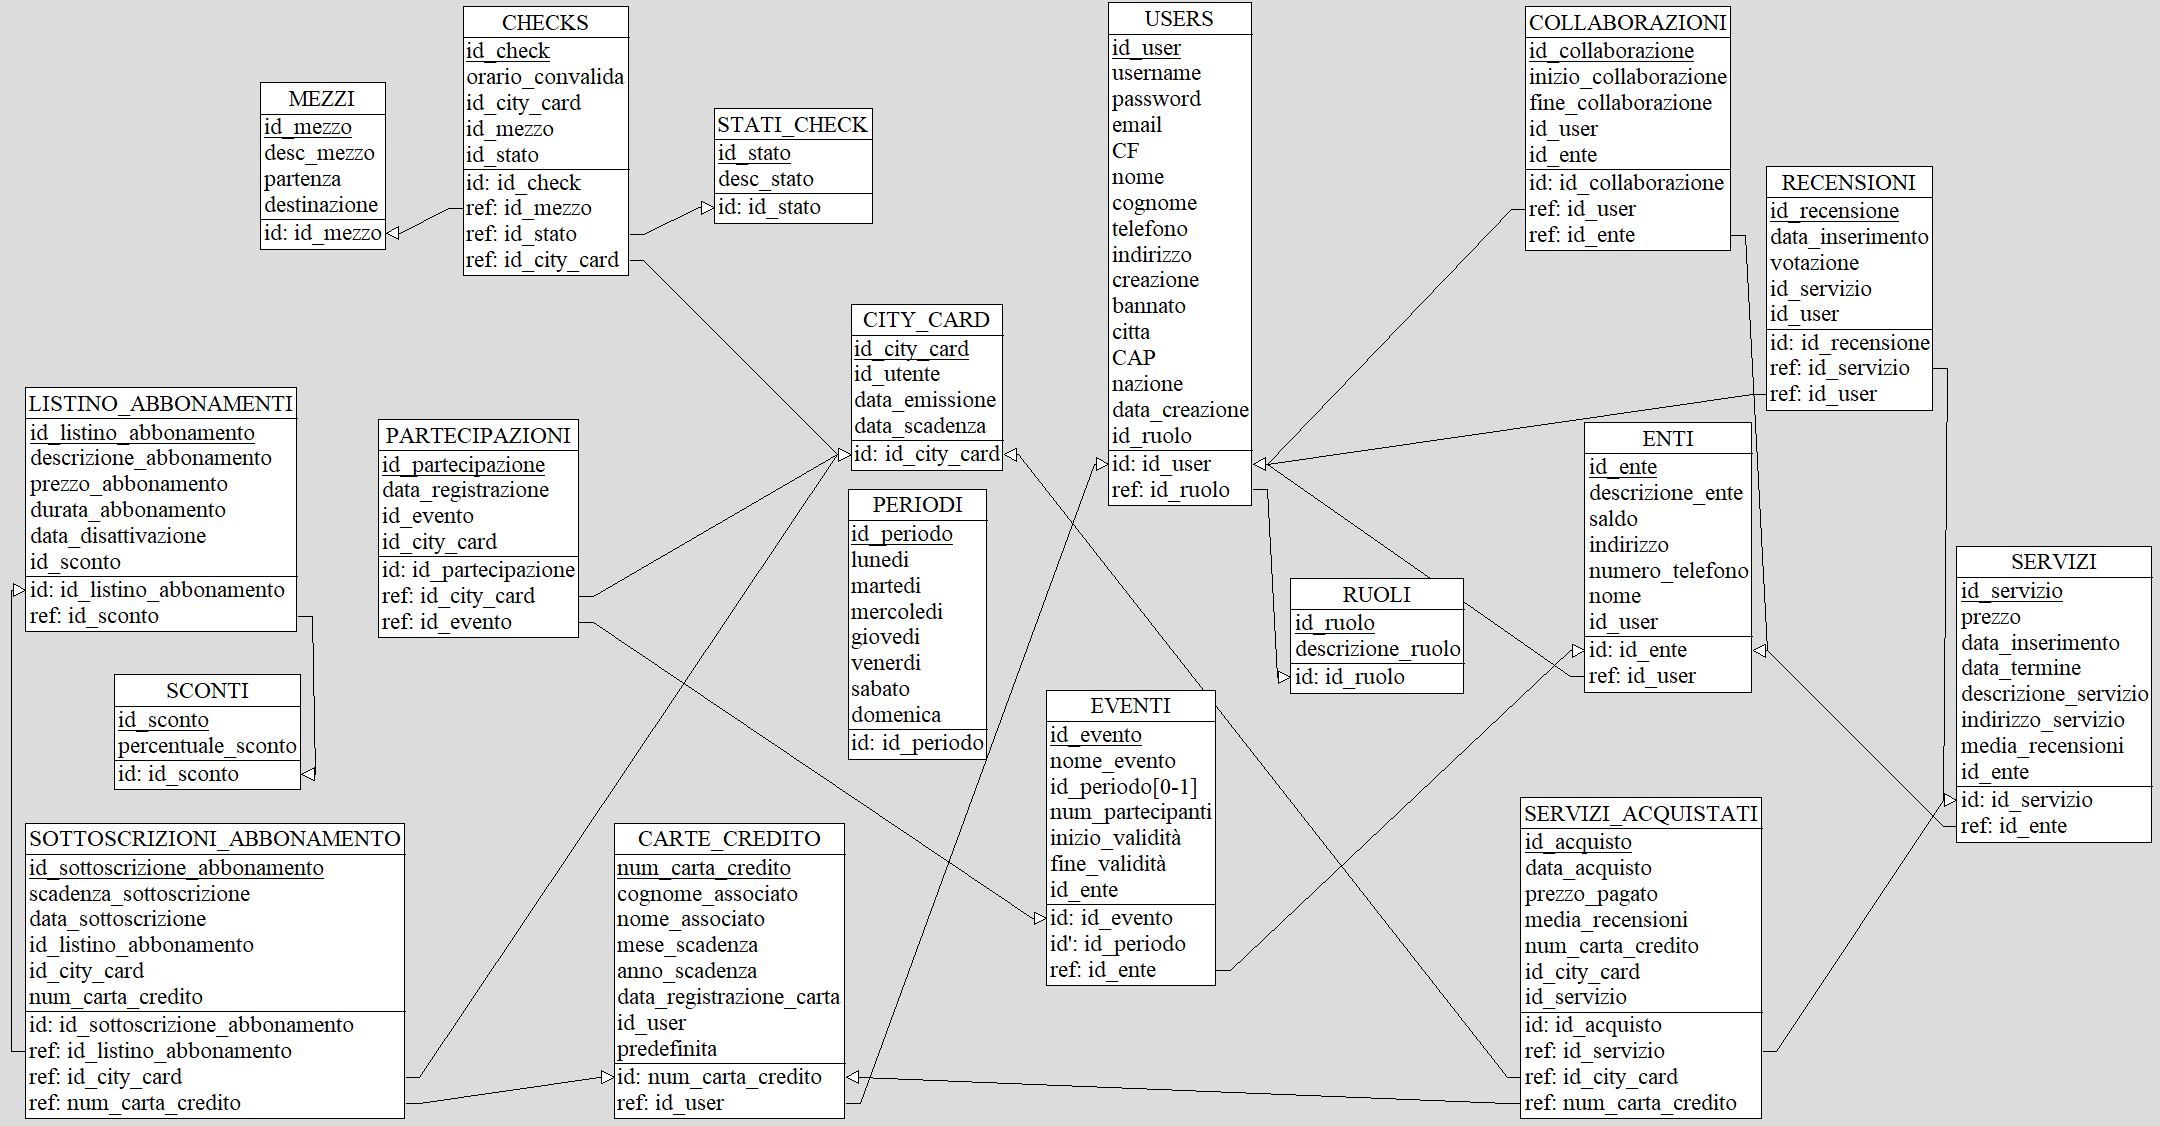
\includegraphics[width=0.9\paperwidth]{schema_logico.png}}
\end{center}

\subsection{Traduzioni delle operazioni in Query SQL}
In questa sezione tradurremo tutte le singole operazioni elementari che abbiamo finora analizzato solo
attraverso gli schemi di navigazione dell’E/R in vere e proprie query in linguaggio SQL. 
Da notare che per facilitare lo dell'applicazione web alcune query sono multiple e di conseguenza è stata posta l'opzione multipleStatements.


\subsubsection{Recuperare tutti gli utenti}

\begin{lstlisting}[language=SQL]
	SELECT id_user, nome, cognome, email, bannato, descrizione_ruolo AS ruolo
	FROM users u
	JOIN ruoli r 
	ON u.id_ruolo = r.id_ruolo;
\end{lstlisting}

\subsubsection{Recuperare tutti gli enti con e senza recensioni}
Seleziona tutti gli enti con e senza recensione, COALESCE restituisce 0 se non c'è una media, i due JOIN imitano una FULL JOIN .
\begin{lstlisting}[language=SQL]
	SELECT e.id_ente, e.nome AS nome_ente, descrizione, e.indirizzo AS indirizzo_ente, numero_telefono, e.id_user, u.nome AS nome_user, cognome, email, cf, telefono, id_ruolo, media_recensioni
	FROM enti e
	JOIN users u
	ON e.id_user = u.id_user
	LEFT JOIN (
	SELECT  s.id_ente AS id_ente,  AVG(COALESCE(votazione, 0)) AS media_recensioni
	FROM recensioni r
	JOIN servizi s
	ON s.id_servizio = r.id_servizio
	GROUP BY s.id_ente
	) AS r
	ON r.id_ente = e.id_ente 
	UNION
	SELECT e.id_ente, e.nome AS nome_ente, descrizione, e.indirizzo AS indirizzo_ente, numero_telefono, e.id_user, u.nome AS nome_user, cognome, email, cf, telefono, id_ruolo, media_recensioni
	FROM enti e
	JOIN users u
	ON e.id_user = u.id_user
	RIGHT JOIN (
	SELECT  s.id_ente AS id_ente,  AVG(COALESCE(votazione, 0)) AS media_recensioni
	FROM recensioni r
	JOIN servizi s
	ON s.id_servizio = r.id_servizio
	GROUP BY s.id_ente
	) AS r
	ON r.id_ente = e.id_ente
\end{lstlisting}


\subsubsection{Recupero lista eventi}
\begin{lstlisting}[language=SQL]
	SELECT ev.*, en.nome AS organizzatore, periodi.*
	FROM eventi ev
	JOIN enti en
	ON ev.id_ente = en.id_ente
	JOIN periodi
	ON periodi.id_periodo = ev.id_periodo
	WHERE now() < ev.fine_validita
	ORDER BY ev.inizio_validita DESC;
\end{lstlisting}

\subsubsection{Recupero lista servizi}
\begin{lstlisting}[language=SQL]
	SET @id_user = ?;     
	SET @cityCard = ( SELECT id_city_card
	FROM city_card
	WHERE id_user = @id_user AND data_scadenza > now());
	SET @percentToPay = (SELECT (100 - sconti.percentuale_sconto) / 100
	FROM sconti 
	JOIN listino_abbonamenti ls 
	ON sconti.id_sconto = ls.id_sconto
	JOIN sottoscrizioni_abbonamento sa
	ON  ls.id_sconto = sa.id_listino_abbonamento
	WHERE sa.id_city_card = @cityCard);
	SELECT se.*, en.nome AS organizzatore, se.prezzo_servizio * @percentToPay AS prezzo_scontato
	FROM servizi se
	JOIN enti en
	ON se.id_ente = en.id_ente
	WHERE now() < se.fine_validita;
\end{lstlisting}

\subsubsection{Recupero acquisti di un utente}
\begin{lstlisting}[language=SQL]
	SELECT sa.data_acquisto, sa.prezzo_pagato, cc.id_city_card, sa.num_carta_credito, servizi.descrizione_servizio AS nome_servizio, u.id_user, sa.id_servizio
	FROM servizi_acquistati sa
	JOIN city_card cc
	ON cc.id_city_card = sa.id_city_card
	JOIN users u
	ON u.id_user = cc.id_user
	JOIN servizi
	ON servizi.id_servizio = sa.id_servizio
	WHERE cc.data_scadenza>now() AND cc.id_user = ?
	ORDER BY sa.data_acquisto DESC;
\end{lstlisting}



\subsubsection{Reitorna statistiche amministratore}
Uso le variabili per rendere più leggibili le query e le unisco in un unico SELECT per rendere l'inserimento in tabelle più semplice. 
\begin{lstlisting}[language=SQL]
	INSERT INTO users (username, nome, cognome, email,
	password, id_ruolo, data_creazione) 
	VALUES (SET @numeroCheckin = (SELECT COUNT(COALESCE(id_check,0)) FROM checks);
	SET @numeroCheckinFalliti = (SELECT COUNT(COALESCE(id_check,0)) FROM checks WHERE id_check != 1);
	SET @numeroCityCardAttive = (SELECT COUNT(COALESCE(id_city_card,0)) FROM city_card WHERE data_scadenza > now());
	SET @numeroEventiAttivi = (SELECT COUNT(COALESCE(id_evento,0)) FROM eventi WHERE fine_validita > now());
	SET @numeroServiziAttivi = (SELECT COUNT(COALESCE(id_servizio,0)) FROM servizi WHERE fine_validita > now());
	
	SELECT 
	@numeroCheckin AS numero_checkin,
	@numeroCheckinFalliti AS numeroCheckinFalliti,
	@numeroCityCardAttive AS numeroCityCardAttive,
	@numeroEventiAttivi AS numeroEventiAttivi,
	@numeroServiziAttivi AS numeroServiziAttivi);
\end{lstlisting}





\subsubsection{Recupero statistiche fornitore}
\begin{lstlisting}[language=SQL]
	SET @id_utente = 2;
	SET @id_ente = ( SELECT c.id_ente
	FROM collaborazioni c
	WHERE c.id_user = @id_utente AND c.fine_collaborazione is null limit 1);
	
	SET @saldo = (SELECT saldo FROM enti WHERE id_ente = @id_ente);
	SET @numeroEventiAttivi = (SELECT COUNT(COALESCE(id_evento,0)) FROM eventi WHERE fine_validita > now() AND id_ente = @id_ente);
	SET @numeroServiziAttivi = (SELECT COUNT(COALESCE(id_servizio,0)) FROM servizi WHERE fine_validita > now() AND id_ente = @id_ente);
	
	
	SELECT  
	IFNULL(@saldo,0) AS saldo,
	@numeroEventiAttivi AS numeroEventiAttivi,
	@numeroServiziAttivi AS numeroServiziAttivi;
\end{lstlisting}




\subsubsection{Recupero listino abbonamenti}
\begin{lstlisting}[language=SQL]
	SELECT l.*, s.percentuale_sconto
	FROM listino_abbonamenti l
	JOIN sconti s
	ON l.id_sconto = s.id_sconto
	WHERE l.data_disattivazione is null or l.data_disattivazione < now();
\end{lstlisting}


\subsubsection{Creazione nuovo ente}
\begin{lstlisting}[language=SQL]
	INSERT INTO enti (nome, descrizione, indirizzo, numero_telefono, id_user) 
	VALUES (?, ?, ?, ?,  ?);
\end{lstlisting}



\subsubsection{Inserimento voto utente}
Dato che un utente può avere una recensione per servizio cancello la inserisco il voto nuovo, calcolo la media, la inserisco nel servizio.
\begin{lstlisting}[language=SQL]
	SET @idUser = ?;
	SET @idServizio = ?;
	
	DELETE 
	FROM recensioni 
	WHERE id_user = @idUser AND id_servizio = @idServizio;
	
	INSERT INTO recensioni (id_user, votazione, id_servizio) VALUES(@idUser,?,@idServizio);
	
	SET @media = (SELECT AVG(votazione) 
	FROM recensioni 
	WHERE id_user = @idUser AND id_servizio = @idServizio);
	
	UPDATE servizi
	SET media_recensioni = @media
	WHERE id_servizio = @idServizio;
\end{lstlisting}



\subsubsection{Reset recensioni di un ente}
Reset di tutte le recensioni riguardanti un ente
\begin{lstlisting}[language=SQL]
	SET @id_ente = ?;
	
	DELETE recensioni 
	FROM recensioni
	JOIN servizi s
	ON s.id_servizio = recensioni.id_servizio
	WHERE s.id_ente = @id_ente;
	
	UPDATE servizi s
	SET media_recensioni = null
	WHERE s.id_ente = @id_ente;
\end{lstlisting}




\subsubsection{Creazione servizio}
Crea un servizio, "LIMIT 1" non dovrebbe servire in quanto un fornitore può essere
associato con solo un ente ma protegge da possibili errori come una doppia scrittura dello stesso record
\begin{lstlisting}[language=SQL]
	INSERT INTO servizi (descrizione_servizio, indirizzo_servizio, id_ente, prezzo_servizio) 
	VALUES (?, ?, 
	( SELECT c.id_ente
	FROM collaborazioni c
	WHERE c.id_user = ? AND c.fine_collaborazione is null LIMIT 1), ?);
\end{lstlisting}

\subsubsection{Registrazione nuovo utente}
\begin{lstlisting}[language=SQL]
	INSERT INTO users (username, nome, cognome, email, password, id_ruolo, data_creazione) 
	VALUES (?,?,?,?,?,?,?);
\end{lstlisting}

\subsubsection{Registrazione nuova carta di credito}
\begin{lstlisting}[language=SQL]
	INSERT INTO carte_credito (num_carta_credito, cognome_associato, nome_associato, mese_scadenza, anno_scadenza, id_user) 
	VALUES (?,?,?,?,?,?);
\end{lstlisting}

\subsubsection{Creazione nuova CityCard}
\begin{lstlisting}[language=SQL]
	INSERT INTO city_card (id_user) 
	VALUES('?');
\end{lstlisting}

\subsubsection{Disattivazione CityCard}
Per disattivare una card pongo la data di scadenza a now().
Per controllare se la card è attiva controllo se il momento di disattivazione è già passato.
In ogni momento un utente può avere al massimo una CityCard attiva,
quindi per default disattivo tutte quelle attive.
\begin{lstlisting}[language=SQL]
	\dfrac{update}{\dfrac{num}{den}} city_card
	SET data_scadenza = now()
	WHERE id_user = ? AND data_scadenza > now();
\end{lstlisting}

\subsubsection{Rendere predefinita una carta di credito}
rendo predefinita una carta di credito di un utente. Rendo non predefinite tutte le altre. Query doppia, una delle alternative a quello fatto in ban
\begin{lstlisting}[language=SQL]
	UPDATE carte_credito
	SET predefinita = 0
	WHERE id_user = ?;
	
	UPDATE carte_credito
	SET predefinita = 1
	WHERE num_carta_credito = ?;
\end{lstlisting}

\subsubsection{Sottoscrizione abbonamento}
\begin{lstlisting}[language=SQL]
	INSERT INTO sottoscrizioni_abbonamento (id_listino_abbonamento, id_city_card, num_carta_credito) 
	VALUES (?, 
	( SELECT id_city_card
	FROM city_card
	WHERE id_user = ? AND data_scadenza > now()), 
	( SELECT num_carta_credito 
	FROM carte_credito
	WHERE id_user = ? AND predefinita = 1));
\end{lstlisting}

\subsubsection{Associa utente a ente}
\begin{lstlisting}[language=SQL]
	INSERT INTO collaborazioni 
	(id_user, id_ente) 
	VALUES (?, ?);
\end{lstlisting}

\subsubsection{Effettua check-in}
\begin{lstlisting}[language=SQL]
	INSERT INTO checks (id_city_card, id_mezzo, id_stato) 
	VALUES (( SELECT id_city_card
	FROM city_card
	WHERE id_user = ? AND data_scadenza > now()), 
	?, ?);
\end{lstlisting}

\subsubsection{Ottieni CityCard di un utente}
\begin{lstlisting}[language=SQL]
	SELECT *, (if (data_scadenza > now(), "attiva", "non attiva")) AS stato
	FROM city_card 
	WHERE id_user = ?
	ORDER BY id_city_card DESC
\end{lstlisting}

\subsubsection{Partecipa a un evento}
\begin{lstlisting}[language=SQL]
	INSERT INTO partecipazioni (id_evento, id_user) VALUES (?,?);
\end{lstlisting}

\subsubsection{Edita Utente}
\begin{lstlisting}[language=SQL]
	UPDATE users 
	SET username = ?, nome = ?, cognome = ?, email = ?, password = ?, indirizzo = ?, telefono = ?, cf = ? 
	WHERE id_user = ?;
\end{lstlisting}

\subsubsection{Banna/sbanna utente}
Query tecnicamente sbagliata ma ho provato ad usare il trucco dell'INNER JOIN per aggirare il problema. L'alternativa è fare due query separate ban/unban.
\begin{lstlisting}[language=SQL]
	UPDATE users u
	INNER JOIN users u1 
	ON u.id_user = u1.id_user
	SET u.bannato = CASE
	WHEN (
	(
	SELECT u1.bannato
	WHERE u1.id_user = ?
	) = 1
	) THEN 0
	ELSE 1
	END
	WHERE u.id_user = ?;
\end{lstlisting}

\subsubsection{Cancella carta di credito}
\begin{lstlisting}[language=SQL]
	DELETE FROM carte_credito
	WHERE num_carta_credito = ?;
\end{lstlisting}

\subsubsection{Effettua login}
\begin{lstlisting}[language=SQL]
	SELECT u.*, r.descrizione_ruolo AS ruolo
	FROM users u
	JOIN ruoli r 
	ON u.id_ruolo = r.id_ruolo
	WHERE username = ? AND password = ?;
\end{lstlisting}

\subsubsection{Ritorna, se presente, la CityCard attiva dell'utente}
\begin{lstlisting}[language=SQL]
	SELECT *
	FROM city_card
	WHERE id_user = ? AND data_scadenza > now();
\end{lstlisting}

\subsubsection{Ritorna ente associato all'utente}
\begin{lstlisting}[language=SQL]
	SELECT *
	FROM collaborazioni
	WHERE id_user = ? AND fine_collaborazione is null;
\end{lstlisting}


\subsubsection{Ritorna, se presente, la sottoscrizione attiva attiva dell'utente}
\begin{lstlisting}[language=SQL]
	SELECT sa.* 
	FROM sottoscrizioni_abbonamento sa
	JOIN city_card cc
	ON sa.id_city_card = cc.id_city_card
	JOIN users u
	ON cc.id_user = u.id_user
	WHERE u.id_user = ?;
\end{lstlisting}


\subsubsection{Ritorna lista check-in fatti da un utente}
\begin{lstlisting}[language=SQL]
	SELECT ch.*, sc.descrizione_stato, m.*
	FROM checks ch
	JOIN city_card cc
	ON ch.id_city_card = cc.id_city_card
	JOIN users u
	ON cc.id_user = u.id_user
	JOIN stati_check sc
	ON ch.id_stato = sc.id_stato
	JOIN mezzi m
	ON ch.id_mezzo = m.id_mezzo
	WHERE u.id_user = ?;
\end{lstlisting}


\subsubsection{Recupera enti}
\begin{lstlisting}[language=SQL]
	SELECT * FROM enti
	WHERE nome like ?;
\end{lstlisting}




\subsubsection{Recupera carte di credito di un utente}
\begin{lstlisting}[language=SQL]
	SELECT c.*, u.nome, u.cognome
	FROM carte_credito c
	JOIN users u
	ON c.id_user = u.id_user
	WHERE c.id_user = ?;
\end{lstlisting}


\subsubsection{Compra servizio}
Compra un servizio tenendo conto dello sconto concesso dalla fascia di abbonamento posseduto, poi aggiunge la somma pagata al saldo dell'ente che eroga il servizio.
La query è stata fatta con le variabili perché senza incappava nello stesso problema del ban utente, cioè conflitto in caso di stesso attributi in INSERT E WHERE della stessa query.
\begin{lstlisting}[language=SQL]
	SET @id_user = ?;
	SET @id_servizio = ?;
	SET @idEnte = (
	SELECT enti.id_ente 
	FROM enti
	JOIN servizi
	ON enti.id_ente = servizi.id_ente
	WHERE servizi.id_servizio = @id_servizio);
	SET @creditCard = ( SELECT num_carta_credito 
	FROM carte_credito
	WHERE id_user = @id_user AND predefinita = 1);
	SET @cityCard = (   SELECT id_city_card
	FROM city_card
	WHERE id_user = @id_user AND data_scadenza > now());
	SET @percentToPay = (SELECT (100 - sconti.percentuale_sconto) / 100
	FROM sconti 
	JOIN listino_abbonamenti ls 
	ON sconti.id_sconto = ls.id_sconto
	JOIN sottoscrizioni_abbonamento sa
	ON  ls.id_sconto = sa.id_listino_abbonamento
	WHERE sa.id_city_card = @cityCard);
	SET @paidPrice = (  SELECT prezzo_servizio * @percentToPay
	FROM servizi
	WHERE id_servizio = @id_servizio);
	
	INSERT INTO servizi_acquistati (id_servizio, prezzo_pagato, num_carta_credito, id_city_card) 
	VALUES (@id_servizio, @paidPrice, @creditCard,@cityCard );
	
	UPDATE enti 
	SET saldo = saldo + @paidPrice
	WHERE id_ente = @idEnte;
\end{lstlisting}




\subsubsection{Creazione evento periodico}
Per ottenere l'ultimo ID inserito in periodi una opzione poteva essere l'utilizzo di LAST{\_}INSERT{\_}ID ma questo richiedeva l'attivazione di PersistentConnections al momento della connessione.

\begin{lstlisting}[language=SQL]
	SET @idUser = ?;
	SET @idEnte = ( SELECT c.id_ente
	FROM collaborazioni c
	WHERE c.id_user = @idUser AND c.fine_collaborazione is null limit 1);
	
	INSERT INTO periodi (lunedi, martedi, mercoledi, giovedi, venerdi, sabato, domenica) 
	VALUES (?,?,?,?,?,?,?);
	
	SET @idPeriodo = (SELECT MAX(id_periodo) FROM periodi);
	
	INSERT INTO eventi (id_periodo, nome_evento, id_ente) 
	VALUES (@idPeriodo, ?, @idEnte);
\end{lstlisting}


\subsubsection{Creazione evento occasionale}
\begin{lstlisting}[language=SQL]
	SET @idUser = ?;
	SET @idEnte = ( SELECT c.id_ente
	FROM collaborazioni c
	WHERE c.id_user = @idUser AND c.fine_collaborazione is null limit 1);
	
	INSERT INTO eventi (id_periodo, nome_evento, id_ente) 
	VALUES (1, ?, @idEnte);
\end{lstlisting}



\section{Progettazione dell'applicazione}
\subsection{Descrizione dell'architettura dell'applicazione}
L'interfaccia utente del nostro elaborato è un prototipo di ciò che sarà effettivamente la piattaforma.\\
\begin{center}
    \fbox{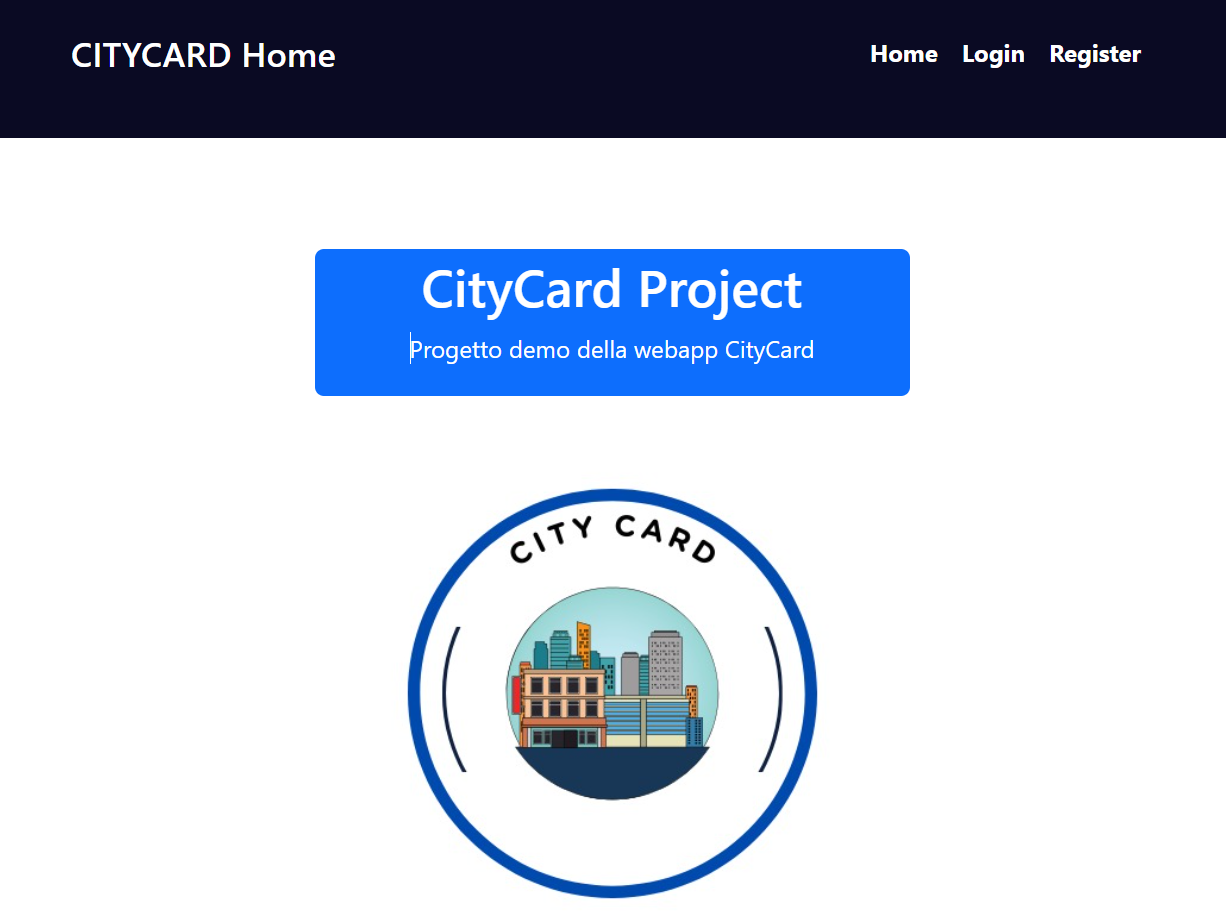
\includegraphics[width=0.95\columnwidth]{home.png}}
\end{center}
L'applicazione è stata realizzata appoggiandosi al framework Node.js. 
I linguaggi utilizzati sono JavaScript per la parte logica e back end, dei fogli di stile CSS e di Bootstrap per quanto concerne l'aspetto grafico. 
Il database è in locale e il DBMS usato è mySQL.
Per la comunicazione con il database è stato utilizzato Express per creare una REST API.\\
\begin{center}
    \fbox{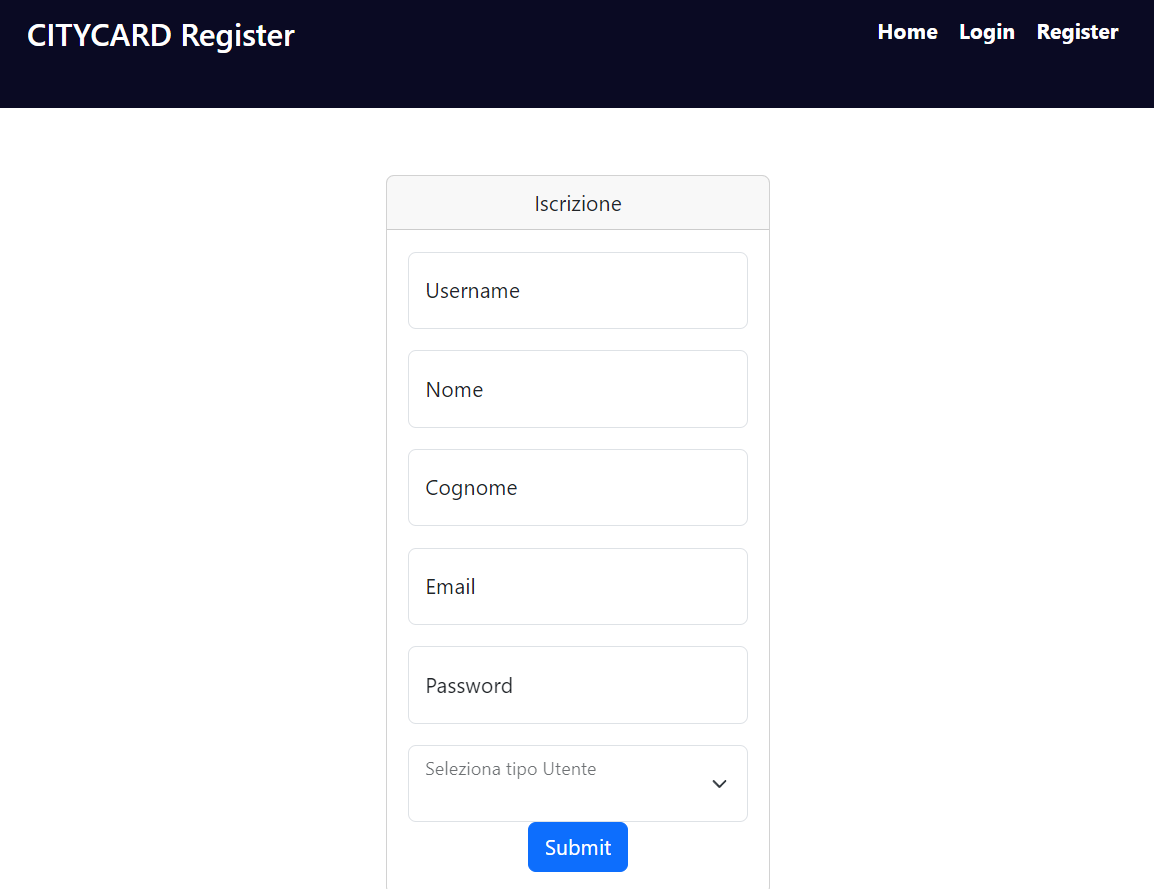
\includegraphics[width=0.95\columnwidth]{register.png}}
\end{center}
Nella schermata iniziale di registrazione sarà possibile, oltre ai dati principali come username e password, il proprio ruolo all'interno del sito.\\
\begin{center}
    \fbox{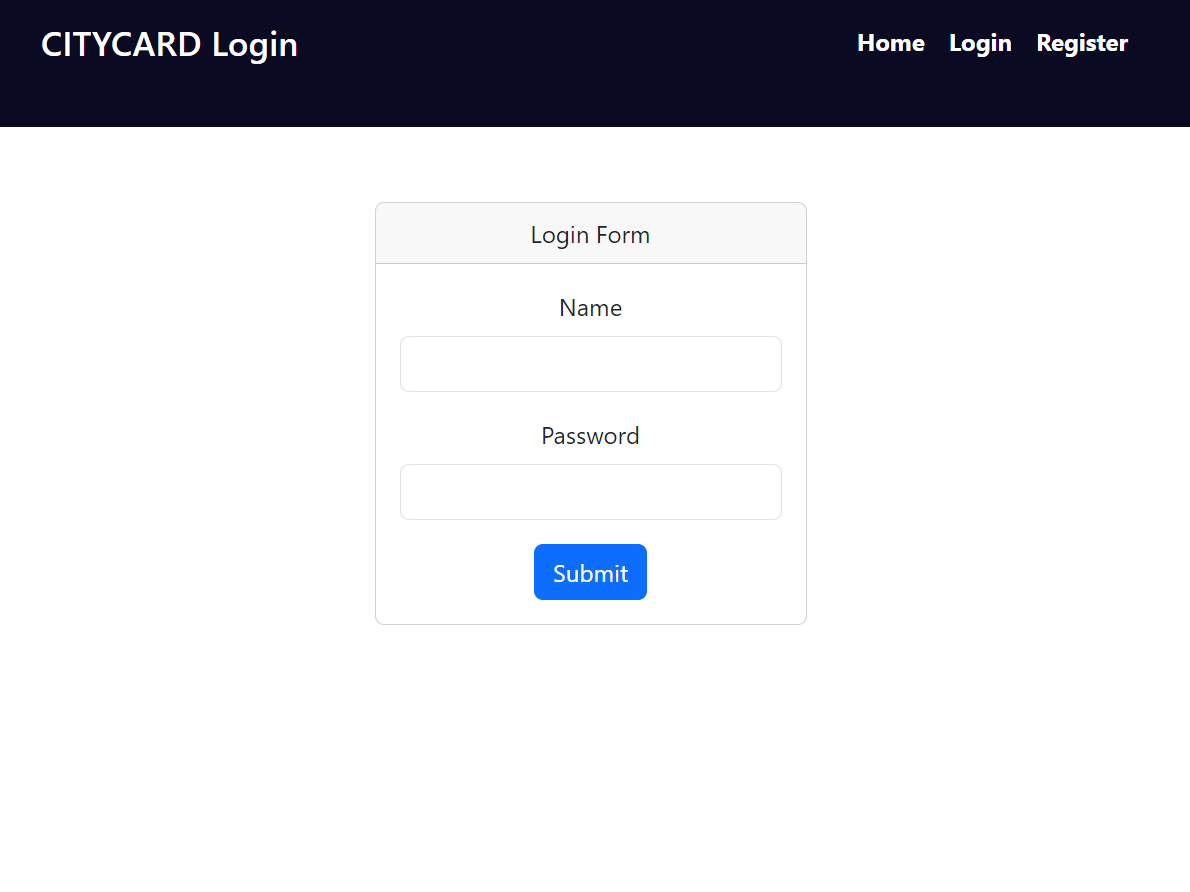
\includegraphics[width=0.95\columnwidth]{login.png}}
\end{center}
Una volta registrato l'utente si potrà loggare nell'applicazione accedendo alla parte dedicata al proprio tipo utente.\\
\vfill
Ci si deve occupare di gestire tre tipologie di utenti: gli amministratori, i fornitori e i clienti.
Passiamo ora ad esaminare questo tipo di interfacce e le diverse funzioni da esse offerte. 

\subsection{L'amministratore}
Una volta effettuato l'accesso l'applicativo offre all'amministratore le seguenti possibilità:
\begin{itemize}
    \item Visualizzare gli enti
    \item Visualizzare gli utenti
    \item Consultazione delle statistiche
    \item Poter tornare indietro al menù principale con il tasto Back
\end{itemize}

Il tasto "Visualizza gli enti" permette di poter visionare l'elenco degli enti registrati all'interno della piattaforma, sarà presente un tasto aggiorna in cui si avrà accesso alla lista più recente delle aziende partner.
La funzione sarà analoga anche per la lsita degli utenti (clienti e fornitori) registrati, sarà inoltre possibile interdire l'accesso al sito tramite il tasto "Banna". Una volta bannato l'utente non potrà più effettuare il login.
Il testo "Back" ci aiuta a tornare al menù principale.


\subsection{Il fornitore}
Una volta effettuato l'accesso come fornitore l'applicativo offre le seguenti possibilità:
\begin{itemize}
    \item Associarsi ad un ente
    \item Creare un ente
    \item Creare un evento
    \item Creare un servizio
    \item Consultazione delle statistiche degli eventi, del saldo e dei servizi
\end{itemize}

Il tasto "Associa al tuo ente" permette al fornitore di potersi associare ad un ente già registrato all'interno della piattaforma mente il tasto "Crea un ente" permette di creare da zero un ente con il quale associarsi.
I successivi comandi permettono di creare un evento o un servizio da far usufruire ai clienti.
La consultazione delle statistiche saldo e servizi permettono rispettivamente di consultare il saldo accumulato dalla registrazione di eventi e dall'acquisto di servizi.
Il tasto "Back" permette di tornare al menù principale.

\subsection{Il cliente}
Se si effettua il primo login in assoluto come cliente gran parte del menù appare disattivato in quanto la maggior parte delle attività si sbloccano in presenza di una CityCard.
Il menù offre le seguenti funzionalità:
\begin{itemize}
    \item Ottieny CityCard
    \item Gestione carte di credito
    \item Sottoscrivi abbonamento
    \item Visualizza eventi
    \item Visualizza servizi
    \item Cronologia acquisti
    \item Simula check in
\end{itemize}
Come detto sopra al momento del primo login le uniche sezioni navigabili sono "Ottieni CityCard" e "Gestione carta di credito" che permettono rispettivamente di ottenere una CityCard e di gestire le carte di credito registrate dal cliente all'interno dell'applicativo.
Una volta ottenuta la tessera sarà disponibile la sezione "Acquista abbonamento" dove sarà possibile scegliere tra tre tipologie di sottoscrizione.  
Una volta scetìlto il tipo di abbonamento anche il resto del menù sarà sbloccato e sarà possibile comprare servizi, prenotarsi ad eventi e visualizzare la cronologia degli acquisti.



\end{document}
